\part{Konveks Optimering}\label{part:konveks}

\chapter{Introduksjon}\label{sec:konveks_intro}

\subsection{Problemformulering}
Konveks optimering handler om å minimere en konveks funksjon under gitte betingelser. Dette er et viktig område innen matematisk optimering og har mange anvendelser i ingeniørfag, økonomi, maskinlæring og mer.

Et generelt betinget optimeringsproblem kan skrives som:
\begin{mini*}
	{x \in \mathbb{R}^n}{f(x)}{}{}
	\addConstraint{g_i(x)}{\leq 0,\quad}{ i = 1,\ldots,m}
	\addConstraint{h_j(x)}{= 0,\quad}{ j = 1,\ldots,p}
\end{mini*}

Her betyr:
\begin{itemize}
	\item \( f(x) \): Målfunksjonen som skal minimeres.
	\item \( g_i(x) \): Ulikhetsbetingelser som setter øvre grenser.
	\item \( h_j(x) \): Likhetsbetingelser som må oppfylles nøyaktig.
\end{itemize}

Disse restriksjonene definerer området, \( \Omega \), der løsningen må ligge.

\subsubsection{Lineært Betinget Optimeringsproblem}

\begin{definition}{Lineært optimeringsproblem}{linear_programming}
	Et lineært optimeringsproblem har formen:
	\begin{mini*}
		{x\in\R^n}{c^Tx}{}{}
		\addConstraint{Ax}{\leq b,}{}
		\addConstraint{Dx}{= e,}{}
	\end{mini*}
	Her er:
	\begin{itemize}
		\item \(c \in \R^n\): Kostnadsvektor.
		\item \(A \in \R^{m \times n}\): Matrise for ulikhetsbetingelsene.
		\item \(D \in \R^{p \times n}\): Matrise for likhetsbetingelsene.
		\item \(b \in \R^m\) og \(e \in \R^p\): Vektorer med høyre siden-verdier.
	\end{itemize}
\end{definition}

\begin{example}{Lineær funksjon}{linear_function}
	La \(f(\symbf{x}) = c^T\symbf{x} + d\) være en lineær funksjon, hvor \(c\) er en vektor normal til en hyperplan og \(d\) er en konstant. Likningen \(f(\symbf{x}) = 0\) definerer da et hyperplan i \(\R^n\).
\end{example}

\begin{example}{Lineær regresjon}{linear_regression}
	Anta at \(X \in \R^{n \times m}\) representerer observasjonsdata og \(y \in \R^n\) representerer måledata. Lineær regresjon kan sees som et lineært optimeringsproblem der vi ønsker å finne vektoren \(w \in \R^m\) som minimerer kvadratavviket:
	\begin{equation*}
		\min_{w \in \R^m} \norm{Xw - y}_2^2.
	\end{equation*}
\end{example}

\subsection{Typer Betingelser}

\subsubsection{Likhetsbetingelser}
Likhetsbetingelser krever at funksjonen oppfyller en eksakt verdi:
\begin{equation*}
	h_j(x) = 0, \quad j = 1,\ldots,p.
\end{equation*}

Geometrisk representerer hver likhetsbetingelse et hyperplan (en \((n-1)\)-dimensjonal flate) i \( \mathbb{R}^n \). For å være i \( \Omega \) må punktet ligge på skjæringspunktet av alle slike flater.

\subsubsection{Ulikhetsbetingelser}
Ulikhetsbetingelser krever at funksjonen ikke overskrider en grense:
\begin{equation*}
	g_i(x) \leq 0, \quad i = 1,\ldots,m.
\end{equation*}

Hver ulikhetsbetingelse definerer et halvrom i \( \mathbb{R}^n \). Et punkt er gyldig dersom det ligger i snittet av alle disse halvrommene. En betingelse \( g_i(x) \leq 0 \) sies å være aktiv ved et punkt \( x^* \) hvis \( g_i(x^*) = 0 \); ellers er den inaktiv.

\section{Tillatte Retninger}
I et tillatt punkt \( x \in \Omega \), kalles en retning \( d \in \mathbb{R}^n \):
\begin{itemize}
	\item En \textbf{tillatt retning} hvis det finnes \( \alpha > 0 \) slik at \( x + td \in \Omega \) for alle \( t \in (0, \alpha] \).
	\item En \textbf{nedstigningsretning} hvis \( \nabla f(x)^T d < 0 \).
\end{itemize}

Den viktige innsikten er at hvis \( d \) er både en tillatt og en nedstigningsretning i \( x \), vil bevegelse langs \( d \) fra \( x \) redusere målfunksjonen samtidig som vi holder oss innenfor den tillatte mengden.

\paragraph{Kjeglen av Tillatte Retninger}
For en konveks mengde \( \Omega \) og et punkt \( x \in \Omega \), er kjeglen av tillatte retninger definert som:
\begin{definition}{Kjeglen av Tillatte Retninger}{cone_of_allowed_directions}

	\[
		\mathcal{F}_\Omega(x) = \{d \in \mathbb{R}^n : \exists \alpha > 0 \text{ s.l. } x + td \in \Omega \text{ for alle } t \in (0, \alpha] \}
	\]
\end{definition}
Denne kjeglen inneholder alle tillatte retninger fra punktet \( x \) i den konvekse mengden \( \Omega \). Den er konveks og lukket, og den kan være tom hvis \( x \) ligger på kanten av \( \Omega \).

\section{Tillatte Områder og Retninger}

\subsection{Det Tillatte Området}
I betingede optimeringsproblemer består det tillatte området \(\Omega\) av alle punkter som tilfredsstiller de gitte betingelsene:
\begin{equation}
	\Omega = \{x \in \mathbb{R}^n \mid g_i(x) \leq 0,\ i = 1,\ldots,m, \text{ og } h_j(x) = 0,\ j = 1,\ldots,p\}.
\end{equation}

Dette settet definerer søkerommet der vi leter etter optimale løsninger. For optimeringsalgoritmer er det avgjørende å forstå den geometriske strukturen til \(\Omega\) og hvordan man navigerer innenfor det.

\subsection{Tillatte Retninger}
Ved et tillatt punkt \(x \in \Omega\), definerer vi:

\begin{definition}{Tillatt Retning}{feasible_direction}
	En vektor \(d \in \mathbb{R}^n\) er en \textbf{tillatt retning} ved \(x\) hvis det finnes \(\alpha > 0\) slik at \(x + td \in \Omega\) for alle \(t \in (0, \alpha]\).
\end{definition}

For glatte betingelser kan vi karakterisere tillatte retninger ved hjelp av gradienter:
\begin{align}
	\nabla g_i(x)^T d & \leq 0 \quad \text{for alle aktive ulikhetsbetingelser } g_i(x) = 0 \\
	\nabla h_j(x)^T d & = 0 \quad \text{for alle likhetsbetingelser } h_j
\end{align}

\subsection{Nedstigningsretninger}
I optimering er vi spesielt interessert i retninger som kan redusere målfunksjonen:

\begin{definition}{Nedstigningsretning}{descent_direction}
	En vektor \(d \in \mathbb{R}^n\) er en \textbf{nedstigningsretning} for funksjon \(f\) ved punkt \(x\) hvis \(\nabla f(x)^T d < 0\).
\end{definition}

Den sentrale innsikten i begrenset optimering er å finne retninger som både er tillatte og nedstigningsretninger. Bevegelse langs slike retninger reduserer målfunksjonen samtidig som den opprettholder gyldighet.

\subsection{Kjeglen av Tillatte Retninger}
For en konveks mengde \(\Omega\) og et punkt \(x \in \Omega\), danner samlingen av alle tillatte retninger et viktig geometrisk objekt:

\begin{definition}{Kjeglen av Tillatte Retninger}{cone_of_feasible_directions}
	\[
		\mathcal{F}_\Omega(x) = \{d \in \mathbb{R}^n : \exists \alpha > 0 \text{ slik at } x + td \in \Omega \text{ for alle } t \in (0, \alpha] \}
	\]
\end{definition}

Denne kjeglen har viktige egenskaper:
\begin{itemize}
	\item Den er alltid konveks
	\item Den er lukket under positiv skalering
	\item Den karakteriserer den lokale geometrien til \(\Omega\) ved \(x\)
	\item Den kan være tom hvis \(x\) er på randen av \(\Omega\) med betingelser som forhindrer bevegelse
\end{itemize}

\subsection{Optimalitetsbetingelser ved bruk av Tillatte Retninger}
En nødvendig betingelse for at \(x^*\) skal være en lokal minimerer er:
\begin{equation}
	\nabla f(x^*)^T d \geq 0 \quad \text{for alle } d \in \mathcal{F}_\Omega(x^*)
\end{equation}

Dette generaliserer standard førsteordensbetingelse \(\nabla f(x^*) = 0\) fra ubegrenset optimering og danner grunnlaget for mange algoritmer for begrenset optimering.

\section{Egenskaper ved konvekse problemer}

Hvis et optimeringsproblem er konvekst, kan vi være sikre på at vi finner en global optimal løsning. Et konvekst optimeringsproblem har følgende egenskaper:
\begin{itemize}
	\item Målfunksjonen \( f \) er konveks
	\item Likhetsbetingelsene \( h_j \) er lineære (affine)
	\item Ulikhetsbetingelsene \( g_i \) er konvekse
\end{itemize}

Konvekse optimeringsproblemer har flere fordelaktige egenskaper:
\begin{itemize}
	\item Ethvert lokalt minimum er også et globalt minimum
	\item KKT-betingelsene er både nødvendige og tilstrekkelige for optimalitet
	\item Det finnes effektive algoritmer for å løse konvekse problemer
\end{itemize}

\chapter{Teori}\label{chap:konveks_teori}

Konveksitet er avgjørende i optimering av flere viktige grunner:

\begin{itemize}
	\item \textbf{Global Optimalitet}: Konvekse optimeringsproblemer har et unikt globalt minimum hvis streng konveksitet holder, siden ethvert lokalt minimum er globalt.

	\item \textbf{Forenklede Optimalitetsbetingelser}: Førsteordens optimalitetsbetingelser er tilstrekkelige for global optimalitet, noe som forenkler analyse og løsningsmetoder.

	\item \textbf{Algoritmisk Effektivitet}: Det finnes effektive algoritmer for å løse konvekse optimeringsproblemer, inkludert gradientmetoder, indrepunktsmetoder og proksimalmetoder.

	\item \textbf{Praktiske Anvendelser}: Mange praktiske problemer innen maskinlæring, kontrollteori, signalbehandling og finans kan formuleres som konvekse optimeringsproblemer eller tilnærmes av dem.

	\item \textbf{Dualitetsteori}: Konveksitet muliggjør kraftige dualitetsresultater som gir alternative løsningsmetoder og sensitivitetsanalyse.
\end{itemize}

Konvekse mengder og funksjoner spiller en sentral rolle i optimering fordi de gir problemer som er relativt enkle å analysere og (ofte) mye enklere å løse, både teoretisk og algoritmisk.
Den viktige egenskapen om at \emph{lokale minima er globale} gjør det mulig å forenkle beregningene betydelig og gir sterke konvergensegenskaper for standardalgoritmer som gradientmetoder, indrepunktsmetoder, subgradientmetoder, og så videre.

\section{Konvekse Mengder}

\begin{definition}{Konveks Mengde}{convex_set}
	En mengde \( C \subset \mathbb{R}^n \) er \textbf{konveks} hvis for ethvert par punkter \( x, y \in C \),
	ligger hele linjesegmentet som forbinder dem også i \( C \). Matematisk kan dette uttrykkes som:
	\[
		x, y \in C, \; \alpha \in [0, 1] \quad \Rightarrow \quad \alpha x + (1-\alpha) y \in C
	\]

	Med andre ord, enhver konveks kombinasjon av punkter i \( C \) forblir i \( C \).
\end{definition}
\begin{figure}[H]
	\centering
	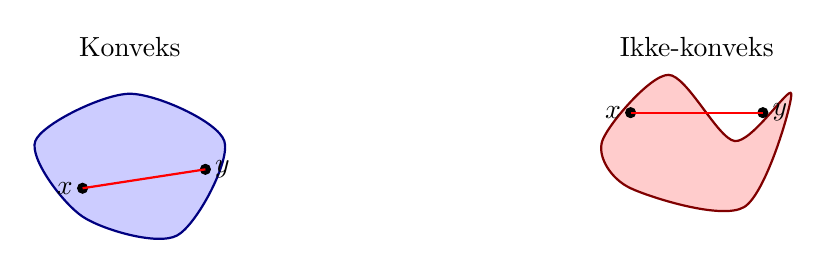
\begin{tikzpicture}[scale=1.2]
		% Convex set (left)
		\begin{scope}[xshift=-3cm]
			\draw[fill=blue!20, draw=blue!50!black, thick] plot[smooth cycle] coordinates {(0,0) (1,0.5) (2,0) (1.5,-1) (0.5,-0.8)};
			\filldraw[black] (0.5,-0.5) circle (1.5pt) node[left] {$x$};
			\filldraw[black] (1.8,-0.3) circle (1.5pt) node[right] {$y$};
			\draw[red, thick] (0.5,-0.5) -- (1.8,-0.3);
			\node at (1,1) {Konveks};
		\end{scope}

		% Non-convex set (right)
		\begin{scope}[xshift=3cm]
			\draw[fill=red!20, draw=red!50!black, thick] plot[smooth cycle] coordinates {(0,0) (0.7,0.7) (1.4,0) (2,0.5) (1.5,-0.7) (0.3,-0.5)};
			\filldraw[black] (0.3,0.3) circle (1.5pt) node[left] {$x$};
			\filldraw[black] (1.7,0.3) circle (1.5pt) node[right] {$y$};
			\draw[red, thick] (0.3,0.3) -- (1.7,0.3);
			\node at (1,1) {Ikke-konveks};

			% Show the part of line segment outside the set
			\draw[red, thick, dashed] (0.8,0.3) -- (1.2,0.3);
		\end{scope}
	\end{tikzpicture}
	\caption{Illustrasjon av konvekse og ikke-konvekse mengder. For en konveks mengde (venstre)
		ligger hele linjesegmentet mellom to punkter i mengden. For en ikke-konveks mengde (høyre)
		finnes det punkter $x$ og $y$ hvor deler av linjesegmentet mellom dem ligger utenfor mengden.}
	\label{fig:convex_nonconvex}
\end{figure}
\begin{example}{Vanlige Konvekse Mengder}{common_convex_sets}
	\begin{itemize}
		\item \textbf{Tomme og Enslige Mengder}: Den tomme mengden $\emptyset$ og ethvert enkeltpunkt $\{x_0\}$ er trivielt konvekse.

		\item \textbf{Affine Mengder}: Alle affine mengder er konvekse, inkludert:
		      \begin{itemize}
			      \item Linjer: $\{x_0 + tv : t \in \mathbb{R}\}$ for fast $x_0$ og $v \neq 0$
			      \item Affine underrom: $\{x : Ax = b\}$ for matrise $A$ og vektor $b$
		      \end{itemize}

		\item \textbf{Euklidske Baller og Sfærer}:
		      \begin{itemize}
			      \item Lukket ball: $B(x_0, r) = \{x : \|x - x_0\| \leq r\}$
			      \item Åpen ball: $B^\circ(x_0, r) = \{x : \|x - x_0\| < r\}$
			      \item Merk: Sfæren $\{x : \|x - x_0\| = r\}$ er \emph{ikke} konveks for $n > 1$
		      \end{itemize}

		\item \textbf{Halvrom og Hyperplan}:
		      \begin{itemize}
			      \item Lukket halvrom: $\{x : a^T x \leq b\}$
			      \item Åpent halvrom: $\{x : a^T x < b\}$
			      \item Hyperplan: $\{x : a^T x = b\}$
		      \end{itemize}

		\item \textbf{Polyedre}: En mengde definert av et endelig antall lineære ulikheter og likheter:
		      \[
			      P = \{x : Ax \leq b, Cx = d\}
		      \]
		      der ulikhetene forstås komponentvis.
	\end{itemize}

\end{example}

\begin{example}{Avanserte Konvekse Mengder}{advanced_convex_sets}
	\begin{itemize}
		\item \textbf{Kjegler}: En mengde $C$ er en konveks kjegle hvis for alle $x \in C$ og $\theta \geq 0$, $\theta x \in C$. Formelt:
		      \[
			      x \in C, \; \theta \geq 0 \quad \Rightarrow \quad \theta x \in C
		      \]

		\item \textbf{Norm-baller}: For enhver norm $\|\cdot\|$ på $\mathbb{R}^n$, er mengden
		      $\{x : \|x\| \leq r\}$ en konveks mengde. Dette inkluderer:
		      \begin{itemize}
			      \item $L_1$-ball: $\{x : \sum_{i=1}^n |x_i| \leq r\}$
			      \item $L_2$-ball (Euklidsk): $\{x : \sqrt{\sum_{i=1}^n x_i^2} \leq r\}$
			      \item $L_\infty$-ball: $\{x : \max_i |x_i| \leq r\}$
		      \end{itemize}

		\item \textbf{Ellipsoider}: En ellipsoide kan representeres som:
		      \[
			      \mathcal{E} = \{x : (x-x_c)^T P^{-1} (x-x_c) \leq 1\}
		      \]
		      hvor $P$ er en positiv definitt matrise og $x_c$ er senteret.
	\end{itemize}
	\begin{figure}[H]
		\centering
		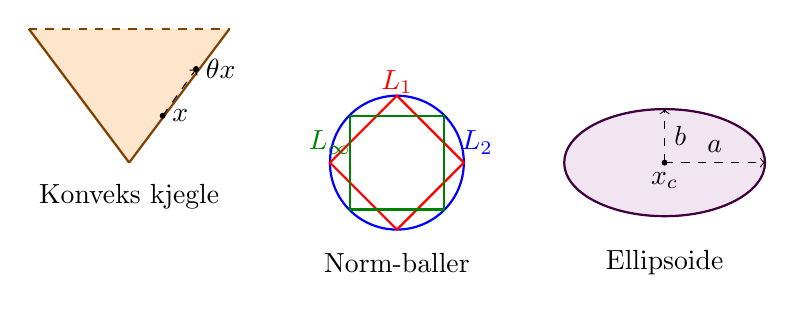
\begin{tikzpicture}[scale=0.85]
			% Convex cone
			\begin{scope}[xshift=-4cm]
				\fill[orange!20] (0,0) -- (1.5,2) -- (-1.5,2) -- cycle;
				\draw[thick, orange!50!black] (0,0) -- (1.5,2);
				\draw[thick, orange!50!black] (0,0) -- (-1.5,2);
				\draw[thick, orange!50!black, dashed] (-1.5,2) -- (1.5,2);
				\node at (0,-0.5) {Konveks kjegle};

				% Scaling illustration
				\filldraw[black] (0.5,0.7) circle (1pt) node[right] {$x$};
				\filldraw[black] (1,1.4) circle (1pt) node[right] {$\theta x$};
				\draw[->, dashed] (0.5,0.7) -- (1,1.4);
			\end{scope}

			% Different norm balls
			\begin{scope}[xshift=0cm]
				% L2 norm (circle)
				\draw[blue, thick] (0,0) circle (1);
				% L1 norm (diamond)
				\draw[red, thick] (1,0) -- (0,1) -- (-1,0) -- (0,-1) -- cycle;
				% L-infinity norm (square)
				\draw[green!50!black, thick] (-0.7,-0.7) rectangle (0.7,0.7);

				\node at (0,-1.5) {Norm-baller};
				\node[blue] at (1.2,0.3) {$L_2$};
				\node[red] at (0,1.2) {$L_1$};
				\node[green!50!black] at (-1,0.3) {$L_\infty$};
			\end{scope}

			% Ellipsoid
			\begin{scope}[xshift=4cm]
				\draw[fill=violet!10] (0,0) ellipse (1.5 and 0.8);
				\draw[thick, violet!50!black] (0,0) ellipse (1.5 and 0.8);
				\filldraw[black] (0,0) circle (1pt) node[below] {$x_c$};
				\draw[->, dashed] (0,0) -- (1.5,0) node[midway, above] {$a$};
				\draw[->, dashed] (0,0) -- (0,0.8) node[midway, right] {$b$};
				\node at (0,-1.5) {Ellipsoide};
			\end{scope}
		\end{tikzpicture}
		\caption{Mer avanserte konvekse mengder: konveks kjegle, norm-baller og ellipsoide.}
		\label{fig:advanced_convex}
	\end{figure}
\end{example}

\subsection{Operasjoner som Bevarer Konveksitet i Mengder}
\begin{theorem}{Konveksitetsbevarende Operasjoner}{convexity_preserving}
	Følgende operasjoner bevarer konveksitet av mengder:
	\begin{itemize}
		\item \textbf{Snitt}: Snittet av enhver samling konvekse mengder er konveks.
		\item \textbf{Lineære eller Affine Avbildninger}: Hvis \( T \) er en lineær (eller affin) transformasjon, og \( C \) er konveks, er \( T(C) \) konveks.
		\item \textbf{Minkowski Sum}: For konvekse \( C_1,C_2 \), er Minkowski-summen \( \{x_1 + x_2 : x_1\in C_1, x_2\in C_2\} \) konveks.
		\item \textbf{Skalering og Translasjon}: For enhver \( \alpha \in \mathbb{R} \) og \( b \in \mathbb{R}^n \), er både \( \alpha C \) og \( C + b \) konvekse.
	\end{itemize}
\end{theorem}

\begin{figure}[H]
	\centering
	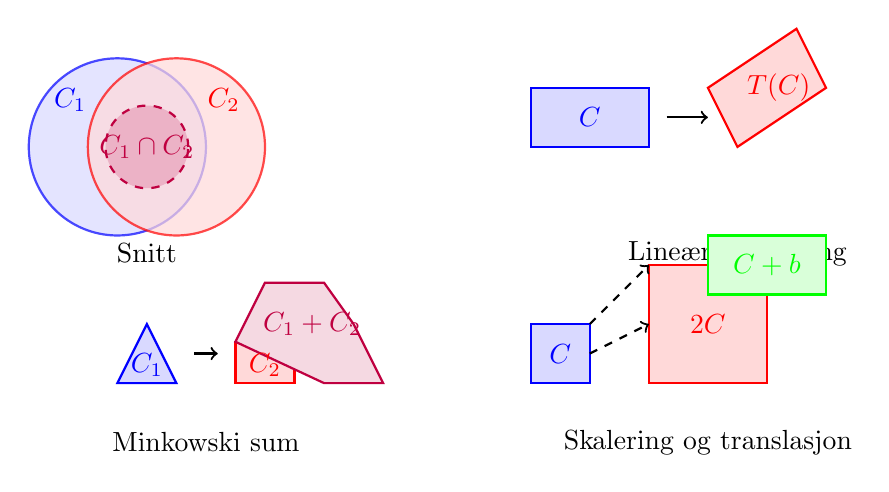
\begin{tikzpicture}[scale=0.75]
		% INTERSECTION
		\begin{scope}[xshift=-4cm, yshift=2cm]
			\draw[blue, thick, fill=blue!15, opacity=0.7] (0,0) circle (1.5);
			\draw[red, thick, fill=red!15, opacity=0.7] (1,0) circle (1.5);
			\fill[purple!30] (0.5,0) circle (0.7);
			\draw[thick, purple, dashed] (0.5,0) circle (0.7);
			\node at (0.5,-1.8) {Snitt};
			\node[blue] at (-0.8,0.8) {$C_1$};
			\node[red] at (1.8,0.8) {$C_2$};
			\node[purple] at (0.5,0) {$C_1 \cap C_2$};
		\end{scope}

		% LINEAR/AFFINE TRANSFORMATION
		\begin{scope}[xshift=3cm, yshift=2cm]
			\draw[blue, thick, fill=blue!15] (0,0) -- (2,0) -- (2,1) -- (0,1) -- cycle;
			\draw[->, thick, black] (2.3,0.5) -- (3,0.5);
			\draw[red, thick, fill=red!15] (3.5,0) -- (5,1) -- (4.5,2) -- (3,1) -- cycle;
			\node at (3.5,-1.8) {Lineær avbildning};
			\node[blue] at (1,0.5) {$C$};
			\node[red] at (4.2,1) {$T(C)$};
		\end{scope}

		% MINKOWSKI SUM
		\begin{scope}[xshift=-4cm, yshift=-2cm]
			\draw[blue, thick, fill=blue!15] (0,0) -- (1,0) -- (0.5,1) -- cycle;
			\draw[red, thick, fill=red!15] (2,0) -- (3,0) -- (3,0.7) -- (2,0.7) -- cycle;
			\draw[purple, thick, fill=purple!15] (3.5,0) -- (4.5,0) -- (4,1) -- (3.5,1.7) -- (2.5,1.7) -- (2,0.7) -- cycle;
			\draw[->, thick, black] (1.3,0.5) -- (1.7,0.5);
			\node[blue] at (0.5,0.3) {$C_1$};
			\node[red] at (2.5,0.3) {$C_2$};
			\node[purple] at (3.3,1) {$C_1 + C_2$};
			\node at (1.5,-1) {Minkowski sum};
		\end{scope}

		% SCALING AND TRANSLATION
		\begin{scope}[xshift=3cm, yshift=-2cm]
			\draw[blue, thick, fill=blue!15] (0,0) -- (1,0) -- (1,1) -- (0,1) -- cycle;
			\draw[red, thick, fill=red!15] (2,0) -- (4,0) -- (4,2) -- (2,2) -- cycle;
			\draw[green, thick, fill=green!15] (3,1.5) -- (5,1.5) -- (5,2.5) -- (3,2.5) -- cycle;
			\draw[->, thick, black, dashed] (1,1) -- (2,2);
			\draw[->, thick, black, dashed] (1,0.5) -- (2,1);
			\node[blue] at (0.5,0.5) {$C$};
			\node[red] at (3,1) {$2C$};
			\node[green] at (4,2) {$C + b$};
			\node at (3,-1) {Skalering og translasjon};
		\end{scope}
	\end{tikzpicture}
	\caption{Illustrasjon av konveksitetsbevarende operasjoner: snitt av konvekse mengder (øverst venstre), lineær avbildning av en konveks mengde (øverst høyre), Minkowski-sum av to konvekse mengder (nederst venstre), og skalering og translasjon av en konveks mengde (nederst høyre).}
	\label{fig:convexity_preserving_operations}
\end{figure}

\subsection{Konveks Kombinasjon}
\begin{definition}{Konveks Kombinasjon}{convex_hull}
	Den konvekse kombinasjonen av en mengde $S$, betegnet $\operatorname{conv}(S)$, er den minste konvekse mengden som inneholder $S$. Matematisk kan den uttrykkes som:
	\[
		\operatorname{conv}(S) = \left\{ \sum_{i=1}^k \theta_i x_i \; \middle| \; k \geq 1, \, x_i \in S, \, \theta_i \geq 0, \, \sum_{i=1}^k \theta_i = 1 \right\}
	\]
	Det vil si mengden av alle konvekse kombinasjoner av punkter i $S$.
\end{definition}

\begin{figure}[H]
	\centering
	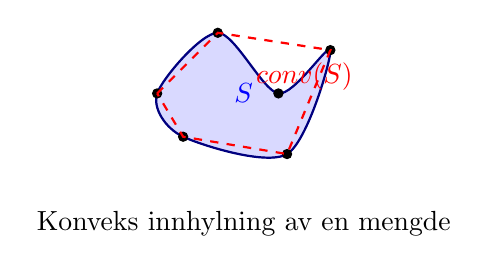
\begin{tikzpicture}[scale=1.1]
		% Non-convex set
		\draw[fill=blue!15] plot[smooth cycle] coordinates {(0,0) (0.7,0.7) (1.4,0) (2,0.5) (1.5,-0.7) (0.3,-0.5)};
		\draw[blue!50!black, thick] plot[smooth cycle] coordinates {(0,0) (0.7,0.7) (1.4,0) (2,0.5) (1.5,-0.7) (0.3,-0.5)};

		% Points in the set
		\filldraw[black] (0,0) circle (1.5pt);
		\filldraw[black] (0.7,0.7) circle (1.5pt);
		\filldraw[black] (1.4,0) circle (1.5pt);
		\filldraw[black] (2,0.5) circle (1.5pt);
		\filldraw[black] (1.5,-0.7) circle (1.5pt);
		\filldraw[black] (0.3,-0.5) circle (1.5pt);

		% Convex hull
		\draw[red, thick, dashed] (0,0) -- (0.7,0.7) -- (2,0.5) -- (1.5,-0.7) -- (0.3,-0.5) -- cycle;

		\node at (1,-1.5) {Konveks innhylning av en mengde};
		\node[blue] at (1,0) {$S$};
		\node[red] at (1.7,0.2) {$\operatorname{conv}(S)$};
	\end{tikzpicture}
	\caption{Den konvekse innhylningen av en mengde er den minste konvekse mengden som inneholder alle punktene i den opprinnelige mengden.}
	\label{fig:convex_hull}
\end{figure}

\subsection{Indre, Rand og Lukking av Konvekse Mengder}

For en konveks mengde $C \subset \mathbb{R}^n$ har vi følgende viktige begreper:

\begin{itemize}
	\item Det \textbf{relative indre} $\operatorname{relint}(C)$ består av punkter som har en full dimensjonal ball (i affin utspent av $C$) rundt seg som ligger i $C$.

	\item Den \textbf{relative randen} $\operatorname{relbd}(C)$ er komplementet til $\operatorname{relint}(C)$ i $C$.

	\item \textbf{Lukkingen} $\operatorname{cl}(C)$ er den minste lukkede mengden som inneholder $C$.
\end{itemize}

\begin{figure}[H]
	\centering
	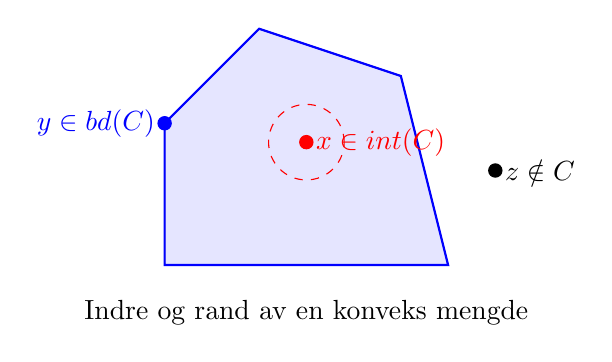
\begin{tikzpicture}[scale=1.2]
		% Draw a convex set (a polygon)
		\draw[fill=blue!10] (0,0) -- (3,0) -- (2.5,2) -- (1,2.5) -- (0,1.5) -- cycle;
		\draw[thick, blue] (0,0) -- (3,0) -- (2.5,2) -- (1,2.5) -- (0,1.5) -- cycle;

		% Interior point
		\filldraw[red] (1.5,1.3) circle (2pt) node[right] {$x \in \operatorname{int}(C)$};
		\draw[red, dashed] (1.5,1.3) circle (0.4);

		% Boundary point
		\filldraw[blue] (0,1.5) circle (2pt) node[left] {$y \in \operatorname{bd}(C)$};

		% Exterior point
		\filldraw[black] (3.5,1) circle (2pt) node[right] {$z \notin C$};

		\node at (1.5,-0.5) {Indre og rand av en konveks mengde};
	\end{tikzpicture}
	\caption{Illustrasjon av indre og rand av en konveks mengde. Punktet $x$ er i det indre og har en ball rundt seg som ligger helt inne i mengden. Punktet $y$ er på randen.}
	\label{fig:interior_boundary}
\end{figure}

Konvekse mengder spiller en sentral rolle i optimeringsteori, spesielt fordi de tillater effektive algoritmer for å finne globale minimumsløsninger av konvekse funksjoner.

\section{Konvekse Funksjoner}

\begin{definition}{Konveks Funksjon}{convex_function}
	En funksjon \( f: C \to \mathbb{R} \), med \( C \subset \mathbb{R}^n \) konveks, er \textbf{konveks} hvis
	\[
		f\bigl(\alpha x + (1-\alpha) y \bigr) \;\le\; \alpha\, f(x) \;+\;(1-\alpha)\, f(y)\quad \text{for alle }x,y \in C,\;\alpha \in [0, 1].
	\]
	Intuitivt ligger grafen til \( f \) "under korden" som forbinder to punkter på grafen.
\end{definition}

\begin{figure}[H]
	\centering
	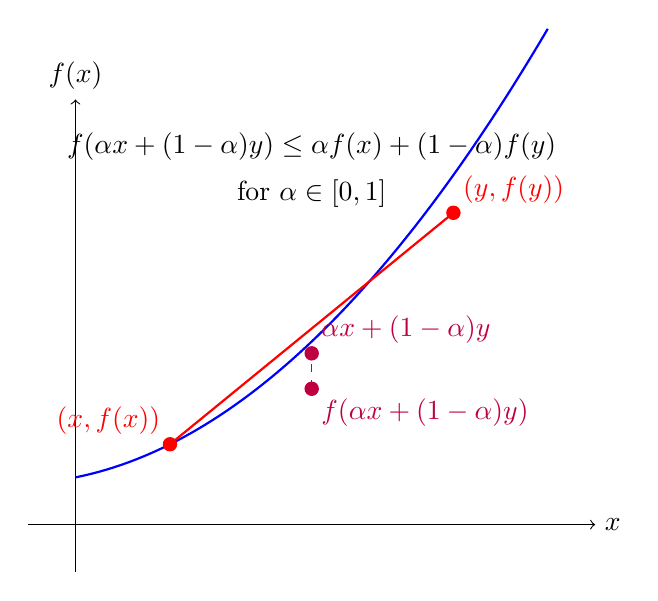
\begin{tikzpicture}[scale=1.2]
		% Koordinatsystem
		\draw[->] (-0.5,0) -- (5.5,0) node[right] {$x$};
		\draw[->] (0,-0.5) -- (0,4.5) node[above] {$f(x)$};

		% Konveks funksjon (parabol)
		\draw[thick, blue, domain=0:5, samples=100] plot (\x, {0.15*\x*\x + 0.2*\x + 0.5});

		% To punkter på funksjonen
		\filldraw[red] (1,0.85) circle (2pt) node[above left] {$(x, f(x))$};
		\filldraw[red] (4,3.3) circle (2pt) node[above right] {$(y, f(y))$};

		% Korde (linjesegment) mellom punktene
		\draw[red, thick] (1,0.85) -- (4,3.3);

		% Konveks kombinasjon-punkt
		\filldraw[purple] (2.5,1.8125) circle (2pt) node[above right] {$\alpha x + (1-\alpha)y$};

		% Vertikal linje fra konveks kombinasjon til funksjonen
		\filldraw[purple] (2.5,1.4375) circle (2pt) node[below right] {$f(\alpha x + (1-\alpha)y)$};
		\draw[purple, dashed] (2.5,1.4375) -- (2.5,1.8125);

		% Tekst som illustrerer ulikheten
		\node at (2.5,4) {$f(\alpha x + (1-\alpha)y) \leq \alpha f(x) + (1-\alpha)f(y)$};
		\node at (2.5,3.5) {for $\alpha \in [0,1]$};
	\end{tikzpicture}
	\caption{Illustrasjon av definisjonen på konveks funksjon. Den røde linjen representerer korden mellom punktene $(x,f(x))$ og $(y,f(y))$. For enhver konveks kombinasjon $\alpha x + (1-\alpha)y$ er funksjonsverdien $f(\alpha x + (1-\alpha)y)$ alltid mindre enn eller lik verdien på korden ved samme punkt.}
	\label{fig:convex_function}
\end{figure}

\subsection{Jensens Ulikhet}
\begin{theorem}{Jensens Ulikhet}{jensens_inequality}
	For enhver konveks funksjon \( f: C \to \mathbb{R} \) og punkter \( x_1, x_2, \ldots, x_k \in C \):
	\[
		f\Bigl(\sum_{i=1}^k \alpha_i x_i \Bigr) \;\le\; \sum_{i=1}^k \alpha_i\, f(x_i),
	\]
	når \( \alpha_i\ge 0 \) og \( \sum_{i=1}^k \alpha_i=1 \).

	For stokastiske variabler, hvis \( X \) er en stokastisk variabel med verdier i \( C \) og \( f \) er konveks, da:
	\[
		f(\mathbb{E}[X]) \leq \mathbb{E}[f(X)]
	\]
	forutsatt at forventningsverdiene eksisterer.
\end{theorem}

\subsection{Subgradienter}
\begin{definition}{Subgradient}{subgradient}
	For en konveks funksjon \( f: C \to \mathbb{R} \), er en vektor \( g \in \mathbb{R}^n \) en \textbf{subgradient} av \( f \) ved \( x \in C \) hvis
	\[
		f(y) \geq f(x) + g^T(y-x), \quad \forall y \in C.
	\]
	Mengden av alle subgradienter av \( f \) ved \( x \) kalles \textbf{subdifferensialet} av \( f \) ved \( x \), og betegnes med \( \partial f(x) \).

	Hvis \( f \) er deriverbar i \( x \), er subgradienten unik og sammenfaller med gradienten, altså \( \partial f(x) = \{\nabla f(x)\} \).
\end{definition}
\begin{figure}[H]
	\centering
	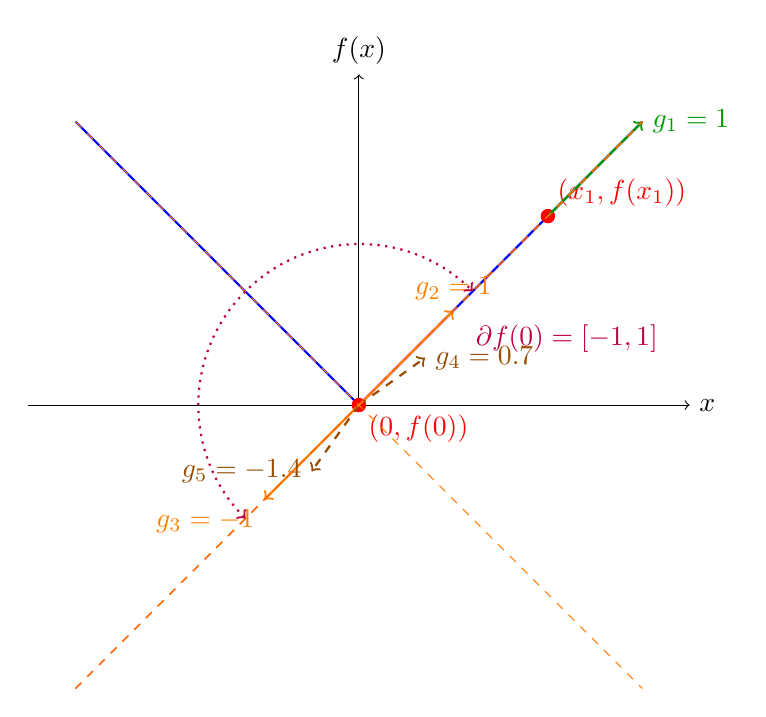
\begin{tikzpicture}[scale=1.2]
		% Koordinatsystem
		\draw[->] (-3.5,0) -- (3.5,0) node[right] {$x$};
		\draw[->] (0,0) -- (0,3.5) node[above] {$f(x)$};

		% Konveks funksjon (stykkevis lineær)
		\draw[thick, blue] plot[domain=-3:0, samples=100] (\x, {-\x});
		\draw[thick, blue] plot[domain=0:3, samples=100] (\x, {\x});

		% Punkt hvor funksjonen ikke er deriverbar
		\filldraw[red] (0,0) circle (2pt) node[below right] {$(0, f(0))$};

		% Differensierbart punkt
		\filldraw[red] (2,2) circle (2pt) node[above right] {$(x_1, f(x_1))$};

		% Subgradient ved differensierbart punkt (entydigt lik gradienten)
		\draw[->, thick, green!60!black] (2,2) -- (3,3) node[right] {$g_1 = 1$};

		% Subgradienter ved ikke-differensierbart punkt (flere mulige)
		\draw[->, thick, orange] (0,0) -- (1,1) node[above] {$g_2 = 1$};
		\draw[->, thick, orange] (0,0) -- (-1,-1) node[below left] {$g_3 = -1$};
		\draw[->, thick, orange!60!black, dashed] (0,0) -- (0.7,0.5) node[right] {$g_4 = 0.7$};
		\draw[->, thick, orange!60!black, dashed] (0,0) -- (-0.5,-0.7) node[left] {$g_5 = -1.4$};

		% Støttende hyperplan ved differensierbart punkt
		\draw[red, dashed] plot[domain=-3:3, samples=2] (\x, {2 + 1*(\x-2)});

		% Støttende hyperplan ved ikke-differensierbart punkt (to eksempler)
		\draw[orange, dashed] plot[domain=-3:3, samples=2] (\x, {0 + 1*(\x-0)});
		\draw[orange, dashed] plot[domain=-3:3, samples=2] (\x, {0 + (-1)*(\x-0)});

		% Subdifferensialet merknad
		\draw[<->, thick, purple, dotted] (-1.2,-1.2) arc (225:45:1.7);
		\node[purple] at (2.2,0.7) {$\partial f(0) = [-1,1]$};
	\end{tikzpicture}
	\caption{Illustrasjon av subgradienter for den konvekse funksjonen $f(x) = |x|$. Ved et differensierbart punkt $(x_1,f(x_1))$ finnes det kun én subgradient (identisk med gradienten). Ved et ikke-differensierbart punkt $(0,f(0))$ består subdifferensialet $\partial f(0)$ av alle verdier i intervallet $[-1,1]$. Hver subgradient definerer et støttende hyperplan (stiplet linje) til epigrafen av $f$.}
	\label{fig:subgradients}
\end{figure}

\begin{example}{Subgradient av L1-normen}{subgradient_example}
	La \( f(x) = \|x\|_1 \). Da er subgradienten ved \( x_0 \) gitt ved:
	\[
		g_i = \begin{cases}
			1       & \text{hvis } x_{0i} > 0 \\
			-1      & \text{hvis } x_{0i} < 0 \\
			[-1, 1] & \text{hvis } x_{0i} = 0
		\end{cases}
	\]
	\begin{figure}[H]
		\centering
		\begin{tikzpicture}
			% Axes
			\draw[->] (-3.5,0) -- (3.5,0) node[right] {\( x \)};
			\draw[->] (0,-1.5) -- (0,3.5) node[above] {\( f(x) \)};

			% L1-norm function
			\draw[thick, blue] plot [domain=-3:3, samples=100] (\x, {abs(\x)});

			% Points on the function
			\filldraw[black] (1,1) circle (2pt) node[below right] {\( x_0 = 1 \)};
			\filldraw[black] (-1,1) circle (2pt) node[above left] {\( x_0 = -1 \)};
			\filldraw[black] (0,0) circle (2pt) node[below left] {\( x_0 = 0 \)};
		\end{tikzpicture}
		\caption{Subgradient av L1-normen ved forskjellige punkter}
		\label{fig:l1_subgradient}
	\end{figure}

\end{example}

\subsection{Epigraf}
Den geometriske tolkningen av konveksitet kan også uttrykkes gjennom epigrafen til en funksjon. Epigrafen er mengden av punkter som ligger over grafen til funksjonen, og gir en visuell representasjon av konveksitet.

\begin{definition}{Epigraf}{epigraph}
	\textbf{Epigrafen} til en funksjon \( f: C \to \mathbb{R} \) er mengden
	\[
		\mathrm{epi}(f) \;=\; \{(x,t)\mid x\in C,\; t\ge f(x)\}.
	\]
	En funksjon \( f \) er konveks hvis og bare hvis \( \mathrm{epi}(f) \) er en konveks mengde i \( \mathbb{R}^{n+1} \).
\end{definition}

\begin{figure}[H]
	\centering
	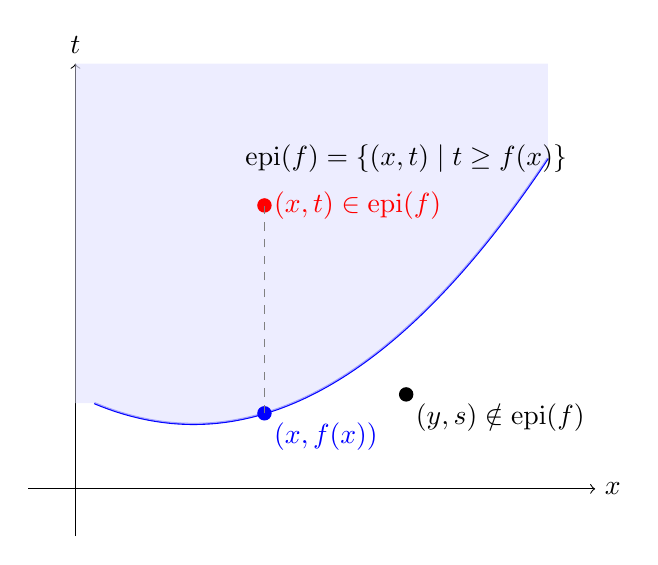
\begin{tikzpicture}[scale=1.2]
		% Koordinatsystem
		\draw[->] (-0.5,0) -- (5.5,0) node[right] {$x$};
		\draw[->] (0,-0.5) -- (0,4.5) node[above] {$t$};

		% Konveks funksjon
		\draw[thick, blue] plot [domain=0.2:5, samples=100] (\x, {0.2*\x*\x - 0.5*\x + 1});

		% Epigraf
		\fill[blue!10, opacity=0.7] (0.2,{0.2*0.2*0.2 - 0.5*0.2 + 1}) --
		plot [domain=0.2:5, samples=100] (\x, {0.2*\x*\x - 0.5*\x + 1}) --
		(5,4.5) -- (0,4.5) -- (0,{0.2*0.2*0.2 - 0.5*0.2 + 1}) -- cycle;

		% Punkter til illustrasjon
		\filldraw[blue] (2,{0.2*2*2 - 0.5*2 + 1}) circle (2pt) node[below right] {$(x, f(x))$};
		\filldraw[red] (2,3) circle (2pt) node[right] {$(x, t) \in \mathrm{epi}(f)$};
		\filldraw[black] (3.5,1) circle (2pt) node[below right] {$(y, s) \notin \mathrm{epi}(f)$};

		% Vertikal linje
		\draw[dashed, gray] (2,{0.2*2*2 - 0.5*2 + 1}) -- (2,3);

		% Merk epigrafet
		\node at (3.5,3.5) {$\mathrm{epi}(f) = \{(x,t) \mid t \geq f(x)\}$};
	\end{tikzpicture}
	\caption{Epigrafen til en konveks funksjon $f$ består av alle punkter $(x,t)$ der $t \geq f(x)$. Dette er det blåskraverte området over grafen til $f$. Et par $(x,t)$ er i epigrafen hvis og bare hvis punktet ligger på eller over funksjonsgrafen.}
	\label{fig:epigraph}
\end{figure}

\subsection{Operasjoner som Bevarer Konveksitet i Funksjoner}

Når vi arbeider med optimering, er det ofte nødvendig å konstruere komplekse målfunksjoner gjennom sammensetning av enklere funksjoner. Det er derfor viktig å forstå hvilke operasjoner som bevarer konveksitet, slik at vi kan være sikre på at resulterende funksjoner fortsatt kan løses effektivt med konvekse optimeringstekniker.

\subsubsection{Algebraiske Operasjoner}
\paragraph{Ikke-negative Vektede Summer}: Hvis \( f_1, f_2, \ldots, f_n \) er konvekse og \( \alpha_1, \alpha_2, \ldots, \alpha_n \geq 0 \), da er \( \sum_{i=1}^n \alpha_i f_i \) konveks.
\begin{proof}[Skisse]
	For alle $x, y \in \text{dom}(f)$ og $\theta \in [0,1]$:
	\begin{align*}
		\sum_{i=1}^n \alpha_i f_i(\theta x + (1-\theta)y) & \leq \sum_{i=1}^n \alpha_i[\theta f_i(x) + (1-\theta)f_i(y)]                  \\
		                                                  & = \theta\sum_{i=1}^n \alpha_i f_i(x) + (1-\theta)\sum_{i=1}^n \alpha_i f_i(y)
	\end{align*}
	hvor den første ulikheten følger av konveksiteten til hver $f_i$.
\end{proof}

\begin{example}{}{}
	Kvadratisk regulert kostfunksjon $f(x) = \|Ax-b\|_2^2 + \lambda\|x\|_2^2$ er konveks fordi den er summen av to konvekse funksjoner med positive koeffisienter.
\end{example}

\subsubsection{Funksjonelle Operasjoner}
\paragraph{Punktvis Maksimum}
Hvis \( f_1, f_2, \ldots, f_n \) er konvekse, da er \( f(x) = \max\{f_1(x), f_2(x), \ldots, f_n(x)\} \) konveks.

\begin{remark}{Punktvis Maksimum Intuisjon}{}
	Maksimumsfunksjonen "arver" den bratteste stigningen til enhver av sine komponentfunksjoner, noe som bevarer konveksitetsegenskapen.
\end{remark}
\begin{example}{}{}
	Hingestap-funksjonen $f(x) = \max\{0, 1-yx\}$, brukt i maskinlæring, er konveks fordi den er maksimum av to konvekse (lineære) funksjoner.
	\begin{figure}[H]
		\centering
		\begin{tikzpicture}[scale=1.0]
			% Hingestap-funksjon
			\draw[domain=-2:2, smooth, thick, blue] plot (\x, {max(0, 1 - \x)}) node[right] {$f(x) = \max(0, 1 - x)$};

			% Akser
			\draw[->] (-2.5,0) -- (2.5,0) node[right] {$x$};
			\draw[->] (0,-1) -- (0,3) node[above] {$f(x)$};
		\end{tikzpicture}
		\caption{Hingestap-funksjonen er konveks fordi den er maksimum av to lineære funksjoner.}
		\label{fig:hinge_loss}
	\end{figure}
\end{example}

\paragraph{Punktvis Supremum}
Hvis \( f_\alpha \) er konveks for hver \( \alpha \in A \), da er \( f(x) = \sup_{\alpha \in A} f_\alpha(x) \) konveks.

Dette er en generalisering av punktvis maksimum til potensielt uendelig mange funksjoner.

\paragraph{Sammensetning med Affin Funksjon}
Hvis \( f \) er konveks og \( g(x) = f(Ax + b) \) hvor \( A \) er en matrise og \( b \) er en vektor, da er \( g \) konveks.

\begin{example}{}{}
	Hvis $f(x) = x^2$ er konveks på $\mathbb{R}$ og $g(x) = f(3x+1) = (3x+1)^2$, da er $g$ også konveks.

	\begin{figure}[H]
		\centering
		\begin{tikzpicture}[scale=1.0]
			% Original function f(x) = x^2
			\draw[domain=-2:2, smooth, thick, blue] plot (\x, {(\x)^2}) node[right] {$f(x) = x^2$};

			% Transformed function g(x) = f(3x+1) = (3x+1)^2
			\draw[domain=-1:1, smooth, thick, red] plot (\x, {(3*\x+1)^2}) node[right] {$g(x) = (3x+1)^2$};

			% Axes
			\draw[->] (-2.5,0) -- (2.5,0) node[right] {$x$};
			\draw[->] (0,0) -- (0,6) node[above] {$y$};
		\end{tikzpicture}
		\caption{Konveksitet bevares under affin transformasjon}
		\label{fig:composition_affine}
	\end{figure}
\end{example}

\paragraph{Minimering over Noen Variabler}
Hvis \( f(x,y) \) er felles konveks i \( (x,y) \), da er \( g(x) = \inf_y f(x,y) \) konveks i \( x \).

Dette resultatet er sentralt i dualitetsteori og Legendre transformasjoner.

\paragraph{Perspektivfunksjonen}
Hvis $f: \mathbb{R}^n \to \mathbb{R}$ er konveks, da er perspektivfunksjonen
$g(x,t) = t \cdot f(x/t)$, definert for $t > 0$, også konveks.

\begin{example}{}{}
	Relativt entropi $g(x,y) = x\log(x/y)$ er konveks for $x,y > 0$ fordi den er perspektivfunksjonen av $f(z) = z\log z$.
	\begin{figure}[H]
		\centering
		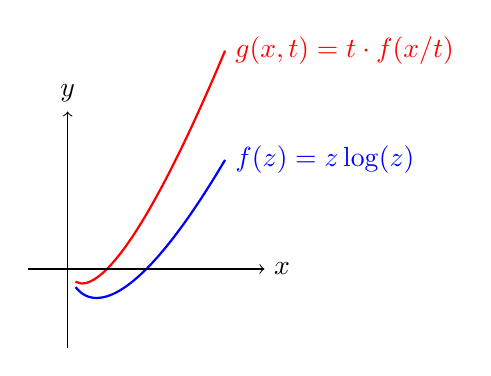
\begin{tikzpicture}[scale=1.0]
			% Original function f(z) = z log(z)
			\draw[domain=0.1:2, smooth, thick, blue] plot (\x, {\x*ln(\x)}) node[right] {$f(z) = z \log(z)$};

			% Perspective function g(x,t) = t * f(x/t)
			\draw[domain=0.1:2, smooth, thick, red] plot (\x, {(\x)*ln(\x/0.5)}) node[right] {$g(x,t) = t \cdot f(x/t)$};

			% Axes
			\draw[->] (-0.5,0) -- (2.5,0) node[right] {$x$};
			\draw[->] (0,-1) -- (0,2) node[above] {$y$};
		\end{tikzpicture}
		\caption{Perspektivfunksjon av en konveks funksjon}
		\label{fig:perspective_function}
	\end{figure}
\end{example}

\paragraph{Sammensetning med Konvekse Funksjoner}
Hvis \( f: \mathbb{R}^n \to \mathbb{R} \) er konveks og \( h: \mathbb{R} \to \mathbb{R} \) er konveks og ikke-avtagende, da er sammensetningsfunksjonen \( g(x) = h(f(x)) \) konveks.

\begin{example}{}{}
	La \( f(x) = x^2 \) og \( h(y) = e^y \). Da er \( g(x) = h(f(x)) = e^{x^2} \) konveks fordi både \( f \) og \( h \) er konvekse.
	\begin{center}
		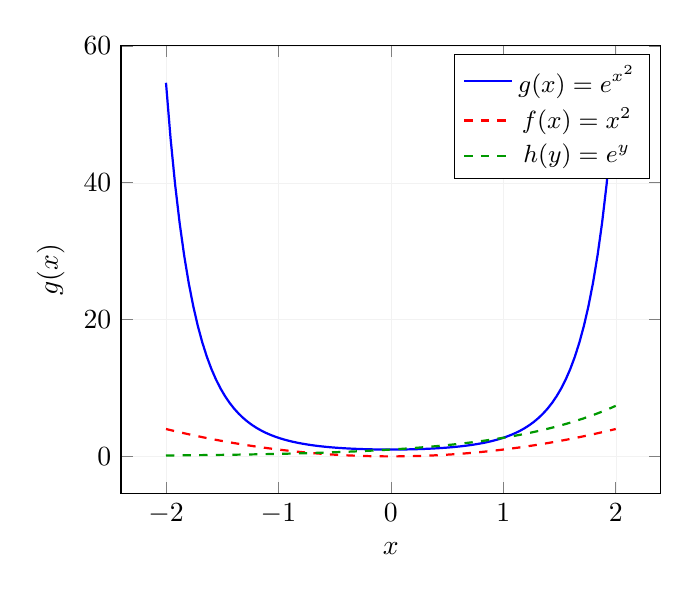
\begin{tikzpicture}
			\begin{axis}[
					domain=-2:2,
					samples=100,
					xlabel=$x$,
					ylabel=$g(x)$,
					legend style={font=\small},
					grid=both,
					grid style={line width=.1pt, draw=gray!10}
				]
				\addplot[blue, thick] {exp(x^2)};
				\addlegendentry{$g(x) = e^{x^2}$}

				\addplot[red, thick, dashed] {x^2};
				\addlegendentry{$f(x) = x^2$}

				\addplot[green!60!black, thick, dashed] {exp(x)};
				\addlegendentry{$h(y) = e^y$}
			\end{axis}
		\end{tikzpicture}
	\end{center}
\end{example}

\begin{figure}[H]
	\centering
	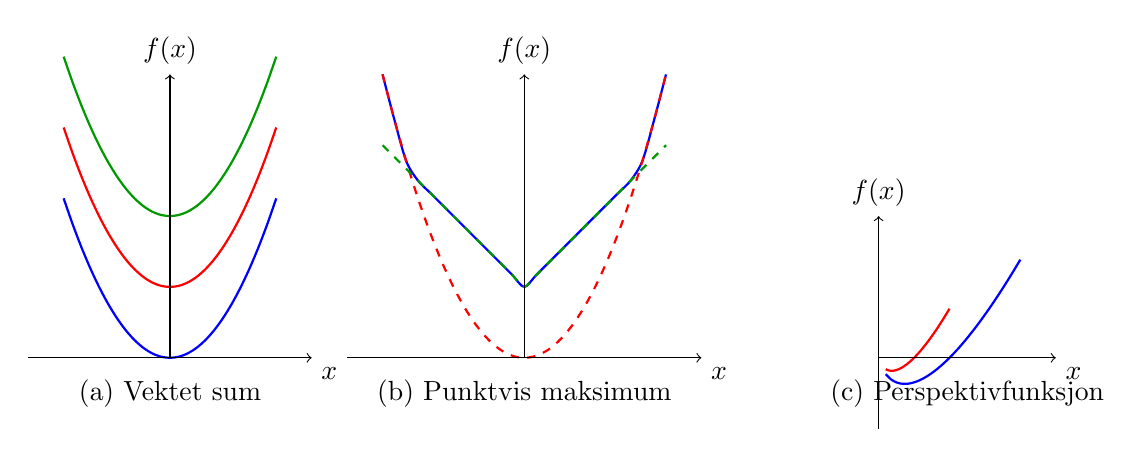
\begin{tikzpicture}[scale=0.9]
		% First function
		\begin{scope}[shift={(-5,0)}]
			\draw[domain=-1.5:1.5, smooth, thick, blue] plot (\x, {(\x)^2});
			\draw[domain=-1.5:1.5, smooth, thick, red] plot (\x, {(\x)^2 + 1});
			\draw[domain=-1.5:1.5, smooth, thick, green!60!black] plot (\x, {(\x)^2 + 2});
			\draw[->] (-2,0) -- (2,0) node[below right] {$x$};
			\draw[->] (0,0) -- (0,4) node[above] {$f(x)$};
			\node at (0,-0.5) {(a) Vektet sum};
		\end{scope}

		% Second function
		\begin{scope}[shift={(0,0)}]
			\draw[domain=-2:2, smooth, thick, blue] plot (\x, {max((\x)^2, 1 + abs(\x))});
			\draw[domain=-2:2, smooth, thick, red, dashed] plot (\x, {(\x)^2});
			\draw[domain=-2:2, smooth, thick, green!60!black, dashed] plot (\x, {1 + abs(\x)});
			\draw[->] (-2.5,0) -- (2.5,0) node[below right] {$x$};
			\draw[->] (0,0) -- (0,4) node[above] {$f(x)$};
			\node at (0,-0.5) {(b) Punktvis maksimum};
		\end{scope}

		% Third function
		\begin{scope}[shift={(5,0)}]
			\draw[domain=0.1:2, smooth, thick, blue] plot (\x, {(\x)*ln(\x)});
			\draw[domain=0.2:2, smooth, thick, red, variable=\t]
			plot ({0.5*\t}, {0.5*\t*ln(0.5*\t/0.5)});
			\draw[->] (0,0) -- (2.5,0) node[below right] {$x$};
			\draw[->] (0,-1) -- (0,2) node[above] {$f(x)$};
			\node at (1.25,-0.5) {(c) Perspektivfunksjon};
		\end{scope}
	\end{tikzpicture}
	\caption{Illustrasjoner av operasjoner som bevarer konveksitet: (a) Vektet sum av konvekse funksjoner, (b) Punktvis maksimum av konvekse funksjoner, (c) Perspektivfunksjon av en konveks funksjon}
	\label{fig:operations_preserving_convexity}
\end{figure}

\section{Konveksitetsekvivalenser}

Følgende tabell oppsummerer ulike måter å karakterisere konvekse funksjoner på:

\begin{table}[H]
	\centering
	\begin{tabular}{|p{3cm}|p{6cm}|p{5cm}|}
		\hline
		\rowcolor{blue!15}
		\textbf{Karakterisering}                                     & \textbf{Matematisk formulering} & \textbf{Intuisjon} \\
		\hline
		\textbf{Definisjon}                                          &
		$f(\theta x + (1-\theta)y) \leq \theta f(x) + (1-\theta)f(y)$ \newline
		for alle $x,y \in \mathcal{D}$, $\theta \in [0,1]$           &
		Funksjonen ligger under linjesegmentet mellom to punkter på grafen                                                  \\
		\hline
		\textbf{Førsteordens betingelse}                             &
		$f(y) \geq f(x) + \nabla f(x)^T(y-x)$ \newline
		for alle $x,y \in \mathcal{D}$                               &
		Funksjonen ligger over alle sine tangentplan                                                                        \\
		\hline
		\textbf{Andreordens betingelse}                              &
		$\nabla^2 f(x) \succeq 0$ for alle $x \in \mathcal{D}$       &
		Hessianen er positiv semidefinitt overalt (krumningen er ikke-negativ i alle retninger)                             \\
		\hline
		\textbf{Epigraf}                                             &
		$\text{epi}(f) = \{(x,t) \in \mathcal{D} \times \mathbb{R} : f(x) \leq t\}$ \newline
		er en konveks mengde                                         &
		Området over grafen er en konveks mengde                                                                            \\
		\hline
		\rowcolor{blue!5}
		\multicolumn{3}{|l|}{\textbf{Avanserte karakteriseringer}}                                                          \\
		\hline
		\textbf{Jensens ulikhet}                                     &
		$f(\mathbb{E}[X]) \leq \mathbb{E}[f(X)]$ \newline
		eller $f(\sum_i \lambda_i x_i) \leq \sum_i \lambda_i f(x_i)$ &
		Forventet verdi av en konveks funksjon er minst like stor som funksjonen evaluert ved forventningsverdien           \\
		\hline
		\textbf{Konveks konjugat}                                    &
		$f^*(y) = \sup_{x} \{y^Tx - f(x)\}$ \newline
		$(f^*)^* = f$ for konvekse, nedre halvkontinuerlige $f$      &
		Legendre-Fenchel transformasjon gir dualitetsrepresentasjon av konvekse funksjoner                                  \\
		\hline
		\textbf{Subgradient}                                         &
		$\partial f(x) = \{g : f(y) \geq f(x) + g^T(y-x) \text{ for alle } y\}$ \newline
		er ikke-tom for alle $x \in \text{int}(\mathcal{D})$         &
		Generaliserer gradient-konseptet til ikke-deriverbare konvekse funksjoner                                           \\
		\hline
	\end{tabular}
	\caption{Ekvivalente karakteriseringer av konvekse funksjoner}
	\label{tab:convexity_equivalences}
\end{table}

\begin{figure}[H]
	\centering
	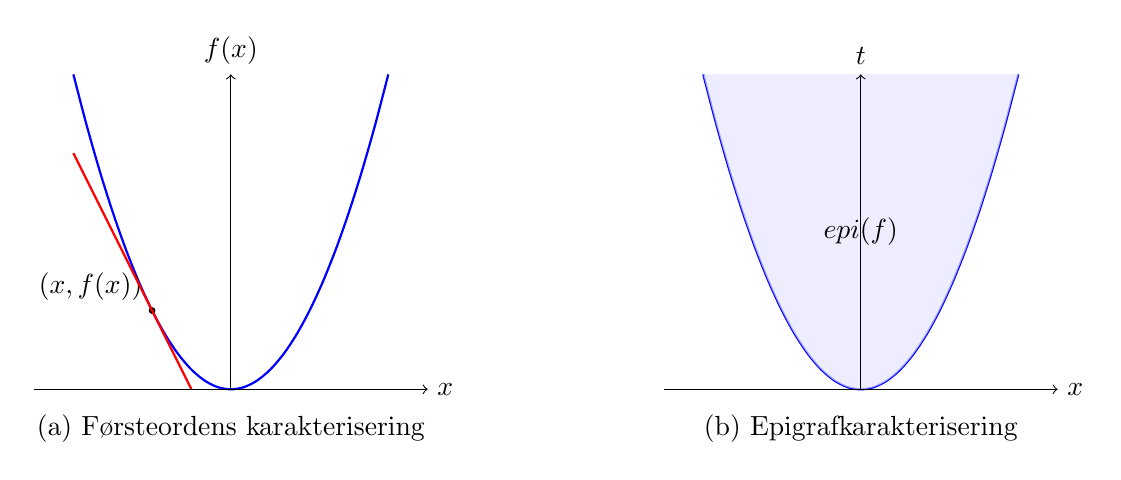
\begin{tikzpicture}[scale=1.0]
		% First-order condition
		\begin{scope}[shift={(-4,0)}]
			% Convex function
			\draw[domain=-2:2, smooth, thick, blue] plot (\x, {(\x)^2});

			% Point on function and tangent
			\filldraw[black] (-1,1) circle (1pt) node[above left] {$(x,f(x))$};
			\draw[red, thick, domain=-2:-0.5] plot (\x, {1 + (-2)*(\x+1)});

			% Axes
			\draw[->] (-2.5,0) -- (2.5,0) node[right] {$x$};
			\draw[->] (0,0) -- (0,4) node[above] {$f(x)$};
			\node at (0,-0.5) {(a) Førsteordens karakterisering};
		\end{scope}

		% Epigraph characterization
		\begin{scope}[shift={(4,0)}]
			% Convex function
			\draw[domain=-2:2, smooth, thick, blue] plot (\x, {(\x)^2});

			% Epigraph
			\fill[blue!10, opacity=0.7]
			(-2,4) --
			plot[domain=-2:2, smooth] (\x, {(\x)^2}) --
			(2,4) -- cycle;

			% Axes
			\draw[->] (-2.5,0) -- (2.5,0) node[right] {$x$};
			\draw[->] (0,0) -- (0,4) node[above] {$t$};
			\node at (0,-0.5) {(b) Epigrafkarakterisering};
			\node at (0,2) {$\text{epi}(f)$};
		\end{scope}
	\end{tikzpicture}
	\caption{To viktige karakteriseringer av konvekse funksjoner: (a) Førsteordens karakterisering: Funksjonen ligger over alle sine tangentplan, (b) Epigrafkarakterisering: Epigrafen til funksjonen er en konveks mengde}
	\label{fig:convexity_characterizations}
\end{figure}
\subsection{Dualitet i Konveks Optimering}
\begin{definition}{Lagrangian-Dualitet}{lagrangian_duality}
	For det konvekse optimeringsproblem
	\begin{mini}
		{x}{f(x)}{}{}
		\addConstraint{g_i(x)}{\leq 0,}{i = 1,\ldots,m}
		\addConstraint{Ax}{= b}{}
	\end{mini}
	er Lagrangian-funksjonen \( \mathcal{L}(x,\lambda,\nu) = f(x) + \sum_{i=1}^m \lambda_i g_i(x) + \nu^T(Ax-b) \) hvor \( \lambda_i \geq 0 \).
	Dualfunksjonen er \( g(\lambda,\nu) = \inf_x L(x,\lambda,\nu) \) og dualproblemet er
	\begin{maxi}
		{\lambda,\nu}{g(\lambda,\nu)}{}{}
		\addConstraint{\lambda}{\geq 0}{}
	\end{maxi}
\end{definition}

\begin{theorem}{Sterk Dualitet}{strong_duality}
	Hvis et konvekst optimeringsproblem tilfredsstiller Slaters betingelse (dvs. det eksisterer et strengt mulig punkt), da gjelder sterk dualitet: de optimale verdiene av primal- og dualproblemet er like.
\end{theorem}

\begin{table}[H]
	\centering
	\begin{tabular}{|p{3cm}|p{5cm}|p{6cm}|}
		\hline
		\rowcolor{blue!25}
		\textbf{Konsept} & \textbf{Definisjon}                                                                   & \textbf{Matematisk Formulering} \\
		\hline
		Konveks Mengde   & En mengde hvor ethvert linjesegment mellom to punkter i mengden ligger helt i mengden &
		\(C\subset \mathbb{R}^n\) er konveks hvis:
		\[\forall x,y\in C,\;\alpha\in [0,1]:\]
		\[\alpha x + (1-\alpha) y\in C\]                                                                                                           \\
		\hline
		\rowcolor{blue!5}
		Konveks Funksjon & En funksjon hvor grafen ligger under linjesegmentet mellom to punkter på grafen       &
		\(f: C \to \mathbb{R}\) er konveks hvis:
		\[f(\alpha x + (1-\alpha) y)\;\le\]\[\alpha f(x) + (1-\alpha) f(y)\]
		for alle \(x,y\in C,\;\alpha\in [0,1]\)                                                                                                    \\
		\hline
	\end{tabular}
	\caption{Grunnleggende konsepter innen konveksitet}
	\label{tab:basic_concepts}
\end{table}

\begin{table}[H]
	\centering
	\begin{tabular}{|p{3cm}|p{5cm}|p{6cm}|}
		\hline
		\rowcolor{rem-color!25}
		\multicolumn{3}{|l|}{\textbf{Karakteriseringer av Konveksitet}}                \\
		\hline
		\rowcolor{rem-color!5}
		1. Ord. Bet. & Tangentapproks. ved ethvert punkt er en global underestimator &
		For deriverbar \(f\), konveksitet er ekvivalent med:
		\[f(y)\;\ge\; f(x) + \nabla f(x)^\mathsf{T} (y - x)\]
		\[\forall x,y \in C\]                                                          \\
		\hline
		2. Ord. Bet. & \(H_f(x)\) er pos. semidefinit overalt i \(C\)                &
		For \(f \in C^2\), konveksitet er ekvivalent med:
		\[\nabla^2 f(x) \succeq 0\quad \forall x \in C\]                               \\
		\hline
	\end{tabular}
	\caption{Karakteriseringer av konveksitet}
	\label{tab:characterizations}
\end{table}

\begin{table}[H]
	\centering
	\begin{tabular}{|p{3cm}|p{5cm}|p{6cm}|}
		\hline
		\rowcolor{cor-color!25}
		\multicolumn{3}{|l|}{\textbf{Viktige Resultater}}                                                                                    \\
		\hline
		\rowcolor{cor-color!5}
		Jensens Ulikhet                                           & Funksjonsverdien av et vektet gjennomsnitt er mindre enn \newline
		eller lik det vektede gjennomsnittet av funksjonsverdiene &
		For konveks \(f\) og vekter \(\alpha_i \geq 0\) med \(\sum_i \alpha_i = 1\):
		\[f\Bigl(\sum_i \alpha_i x_i\Bigr)\;\le\;\sum_i \alpha_i f(x_i)\]                                                                    \\
		\hline
		Epigraf                                                   & Mengden av alle punkter som ligger på eller over grafen til funksjonen &
		\(\mathrm{epi}(f)=\{(x,t) \mid x\in\mathrm{dom}(f), t\ge f(x)\}\)

		\(f\) er konveks \(\Leftrightarrow\) \(\mathrm{epi}(f)\) er konveks                                                                  \\
		\hline
		\rowcolor{cor-color!5}
		Subgradient                                               & Generalisering av gradient for ikke-deriverbare funksjoner             &
		En vektor \(g\) er en subgradient av konveks \(f\) ved \(x\) hvis:
		\[f(y)\;\ge\; f(x) + g^\mathsf{T}(y-x)\quad \forall y \in C\]                                                                        \\
		\hline
	\end{tabular}
	\caption{Viktige resultater innen konveksitet}
	\label{tab:important_results}
\end{table}

\begin{table}[H]
	\centering
	\begin{tabular}{|p{3cm}|p{5cm}|p{6cm}|}
		\hline
		\rowcolor{prop-color!25}
		\multicolumn{3}{|l|}{\textbf{Optimeringsteori}}                                                                            \\
		\hline
		\rowcolor{prop-color!5}
		Lokale/Globale\newline Minima & For konvekse problemer er\newline ethvert lokalt minimum\newline også et globalt minimum &
		For konveks \(f\) på konveks \(C\):\newline\quad\(\text{lokal min} \iff \text{global min}\)                                \\
		\hline
		Sterk Dualitet                & Under visse betingelser er det ingen dualitetsgap                                        &
		Under Slaters betingelse:
		\[\text{primal opt.} = \text{dual opt.}\]                                                                                  \\
		\hline
	\end{tabular}
	\caption{Optimeringsteori og konveksitet}
	\label{tab:optimization_theory}
\end{table}

\section{Eksempler på konvekse funksjoner}

\begin{example}{Vanlige konvekse funksjoner}{common_convex_functions}
	\begin{itemize}
		\item \textbf{Lineære og affine funksjoner:} \( f(x) = c^Tx + \beta \)
		\item \textbf{Normer:} \( f(x) = \|x\|_p \), \( p \geq 1 \)
		\item \textbf{Kvadratiske former:} \( f(x) = x^T Q x \) med \( Q \succeq 0 \)
		\item \textbf{Eksponentialfunksjoner:} \( f(x) = e^{\alpha x} \), \( f(x) = \exp(\langle \alpha, x \rangle) \)
		\item \textbf{Log-barriere:} \( f(x) = -\log(x) \) for \( x > 0 \)
		\item \textbf{Entropifunksjoner:} \( f(x) = x\log(x) \) for \( x > 0 \)
		\item \textbf{Maksimumsfunksjoner:} \( f(x) = \max\{x_1, \dots, x_n\} \)
	\end{itemize}
\end{example}

\begin{table}[H]
	\centering
	\begin{tabular}{|l|l|c|}
		\hline
		\textbf{Funksjon}                          & \textbf{Domene}       & \textbf{Konveksitet} \\
		\hline
		\( f(x) = c^Tx + b \)                      & \( \mathbb{R}^n \)    & Konveks og konkav    \\
		\( f(x) = \|x\|_p \), \( p \geq 1 \)       & \( \mathbb{R}^n \)    & Konveks              \\
		\( f(x) = x^TQx \), \( Q \succeq 0 \)      & \( \mathbb{R}^n \)    & Konveks              \\
		\( f(x) = e^x \)                           & \( \mathbb{R} \)      & Konveks              \\
		\( f(x) = -\log(x) \)                      & \( \mathbb{R}_{++} \) & Konveks              \\
		\( f(x) = x\log(x) \)                      & \( \mathbb{R}_{++} \) & Konveks              \\
		\( f(x) = 1/x \)                           & \( \mathbb{R}_{++} \) & Konveks              \\
		\( f(x) = \max\{x_1, x_2, \ldots, x_n\} \) & \( \mathbb{R}^n \)    & Konveks              \\
		\hline
	\end{tabular}
	\caption{Eksempler på vanlige konvekse funksjoner}
	\label{tab:convex_functions}
\end{table}

\section{Tangent-- og Normal Kjegler}

\subsection{Tangetkjegle}
Tangetkjeglen \(T_{\Omega}(x)\) ved et punkt \(x \in \Omega\) er mengden av alle retninger som kan beskrives som:
\begin{equation*}
	T_{\Omega}(x) = \{d \in \mathbb{R}^n \mid \nabla g_i(x)^T d \leq 0 \text{ for alle aktive } g_i,\ \nabla h_j(x)^T d = 0 \text{ for alle } h_j\}.
\end{equation*}
Dette representerer alle mulige bevegelser innenfor \(\Omega\) fra punktet \(x\).

\subsection{Normalkjegle}
Normalkjeglen \(N_{\Omega}(x)\) er definert som mengden av vektorer som er ortogonale til alle retninger i tangetkjeglen:
\begin{equation*}
	N_{\Omega}(x) = \{v \in \mathbb{R}^n \mid v^T d \leq 0 \text{ for alle } d \in T_{\Omega}(x)\}.
\end{equation*}
Både tangent- og normalkjegle er viktige for å formulere de første ordens nødvendige betingelsene (KKT-betingelsene) som skal diskuteres i neste kapittel.

\section{Separerende og Støttende Hyperplan}

\subsection{Separerende Hyperplan Teorem}
\begin{theorem}{Separerende Hyperplan Teorem}{separating_hyperplane_theorem}
	La \( C \) og \( D \) være disjunkte ikke-tomme konvekse mengder i \( \mathbb{R}^n \). Da gjelder:
	\begin{enumerate}
		\item Hvis \( C \) er åpen, eksisterer det en ikke-null vektor \( a \in \mathbb{R}^n \) og \( b \in \mathbb{R} \) slik at \( a^T x < b \leq a^T y \) for alle \( x \in C \) og \( y \in D \).
		\item Hvis både \( C \) og \( D \) er lukket og minst én er kompakt, eksisterer det en ikke-null vektor \( a \in \mathbb{R}^n \) og konstanter \( b_1, b_2 \in \mathbb{R} \) med \( b_1 < b_2 \) slik at \( a^T x \leq b_1 < b_2 \leq a^T y \) for alle \( x \in C \) og \( y \in D \).
	\end{enumerate}
	I begge tilfeller definerer likningen \(a^Tx = b\) et hyperplan som separerer mengdene \(C\) og \(D\).
\end{theorem}

\begin{figure}[H]
	\centering
	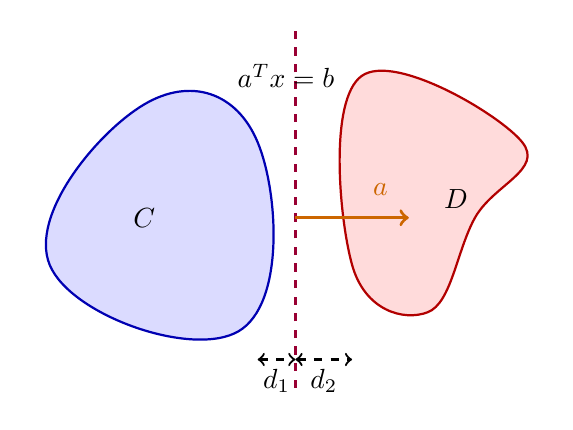
\begin{tikzpicture}[scale=1.2]
		% Første konvekse mengde
		\fill[blue!20, opacity=0.7] plot[smooth cycle, tension=0.8] coordinates {(-2.5,-0.5) (-1.5,1.2) (-0.3,0.8) (-0.5,-1.2)};
		\draw[blue!70!black, thick] plot[smooth cycle, tension=0.8] coordinates {(-2.5,-0.5) (-1.5,1.2) (-0.3,0.8) (-0.5,-1.2)};
		\node at (-1.5,0) {\( C \)};

		% Andre konvekse mengde
		\fill[red!20, opacity=0.7] plot[smooth cycle, tension=0.7] coordinates {(0.8,1.5) (2.5,0.8) (2,0) (1.5,-1) (0.7,-0.5)};
		\draw[red!70!black, thick] plot[smooth cycle, tension=0.7] coordinates {(0.8,1.5) (2.5,0.8) (2,0) (1.5,-1) (0.7,-0.5)};
		\node at (1.8,0.2) {\( D \)};

		% Separerende hyperplan
		\draw[thick, dashed, purple!80!black] (0.1,-1.8) -- (0.1,2);

		% Normalvektor til hyperplanet
		\draw[->, thick, orange!80!black, line width=1.2pt] (0.1,0) -- (1.3,0);
		\node[orange!80!black] at (1.0,0.3) {\( a \)};

		% Hyperplan likning
		\node[black] at (0,1.5) {\( a^T x = b \)};

		% Avstand-notasjoner
		\draw[<->, thick, black, dashed] (-0.3,-1.5) -- (0.1,-1.5);
		\draw[<->, thick, black, dashed] (0.1,-1.5) -- (0.7,-1.5);
		\node[black, below] at (-0.1,-1.5) {$d_1$};
		\node[black, below] at (0.4,-1.5) {$d_2$};
	\end{tikzpicture}
	\caption{Separerende hyperplan mellom to konvekse mengder \( C \) og \( D \). Vektoren \( a \) er normal til hyperplanet og peker mot mengden \( D \). Ved streng separasjon (tilfelle 2 i teoremet) er avstanden \( d_1 + d_2 > 0 \) mellom mengdene positiv.}
	\label{fig:separating_hyperplane}
\end{figure}

\subsection{Støttende Hyperplan}
\begin{definition}{Støttende Hyperplan}{supporting_hyperplane}
	Et \textbf{støttende hyperplan} til en mengde \( C \subset \mathbb{R}^n \) ved et grensepunkt \( x_0 \in \text{bd}(C) \) er et hyperplan som inneholder \( x_0 \) og hvor hele \( C \) ligger på én side av hyperplanet.

	Formelt er hyperplanet definert ved \( a^T x = b \) støttende til \( C \) ved \( x_0 \) hvis:
	\begin{itemize}
		\item \( a^T x_0 = b \) (hyperplanet inneholder punktet \( x_0 \))
		\item Enten \( a^T x \leq b \) for alle \( x \in C \), eller \( a^T x \geq b \) for alle \( x \in C \)
	\end{itemize}
\end{definition}

\begin{theorem}{Eksistens av Støttende Hyperplan}{supporting_hyperplane_existence}
	For enhver ikke-tom konveks mengde \( C \subset \mathbb{R}^n \) og ethvert grensepunkt \( x_0 \in \text{bd}(C) \), eksisterer minst ett støttende hyperplan til \( C \) ved \( x_0 \).
\end{theorem}

\begin{figure}[H]
	\centering
	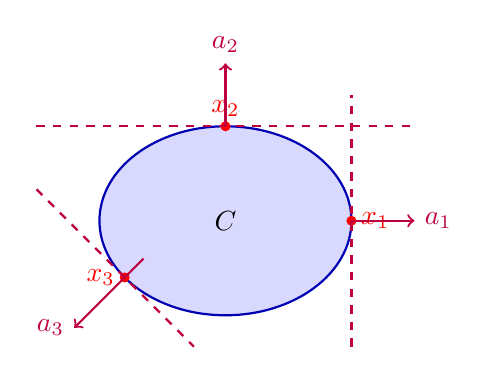
\begin{tikzpicture}[scale=0.8]
		% Konveks mengde (ellipse)
		\fill[blue!15] (0,0) ellipse (2 and 1.5);
		\draw[blue!70!black, thick] (0,0) ellipse (2 and 1.5);
		\node at (0,0) {\( C \)};

		% Grensepunkter
		\filldraw[red] (2,0) circle (2pt) node[right] {\( x_1 \)};
		\filldraw[red] (0,1.5) circle (2pt) node[above] {\( x_2 \)};
		\filldraw[red] (-1.6,-0.9) circle (2pt) node[left] {\( x_3 \)};

		% Støttende hyperplan ved x_1
		\draw[thick, purple, dashed] (2,-2) -- (2,2);
		\draw[->, thick, purple] (2,0) -- (3,0) node[right] {\( a_1 \)};

		% Støttende hyperplan ved x_2
		\draw[thick, purple, dashed] (-3,1.5) -- (3,1.5);
		\draw[->, thick, purple] (0,1.5) -- (0,2.5) node[above] {\( a_2 \)};

		% Støttende hyperplan ved x_3
		\draw[thick, purple, dashed] (-3.0,0.5) -- (-0.5,-2.0);
		\draw[->, thick, purple] (-1.3,-0.6) -- (-2.4,-1.7) node[left] {\( a_3 \)};
	\end{tikzpicture}
	\caption{Støttende hyperplan til en konveks mengde \( C \) ved tre forskjellige grensepunkter. For hvert punkt \( x_i \) viser vektoren \( a_i \) normalen til det støttende hyperplanet, som peker bort fra mengden.}
	\label{fig:supporting_hyperplanes}
\end{figure}

\paragraph{Egenskaper ved støttende hyperplan}
For konvekse mengder har støttende hyperplan flere viktige egenskaper:

\begin{itemize}
	\item For enhver lukket konveks mengde \( C \) og ethvert punkt \( y \notin C \), eksisterer et hyperplan som strengt separerer \( y \) fra \( C \).

	\item Et hyperplan er støttende til en konveks mengde hvis og bare hvis det inneholder minst ett grensepunkt og hele mengden ligger på én side av hyperplanet.

	\item Enhver lukket konveks mengde er snittet av alle lukkede halvrom som inneholder den.

	\item For et grensepunkt til en konveks mengde med glatt grense, er det støttende hyperplanet unikt og tangerer mengden i dette punktet.
\end{itemize}
\begin{example}{Støttende Hyperplan til en Kule}{supporting_hyperplane_ball}
	La \( B = \{x \in \mathbb{R}^n : \|x - c\| \leq r\} \) være en lukket kule med sentrum \( c \) og radius \( r \). For ethvert grensepunkt \( x_0 \) på kulen (der \( \|x_0 - c\| = r \)), er det støttende hyperplanet gitt ved:
	\[
		(x_0 - c)^T (x - x_0) = 0
	\]
	Dette hyperplanet har normalvektor \( a = x_0 - c \) som peker radielt utover fra kulen.

	\begin{figure}[H]
		\centering
		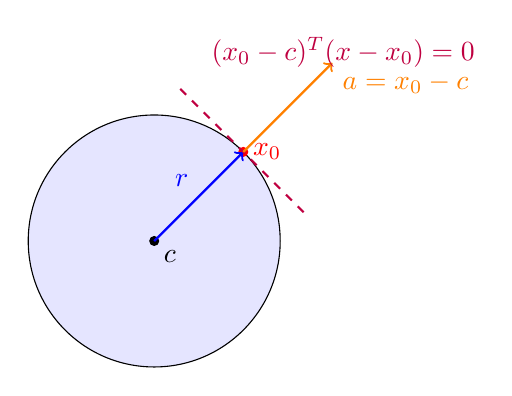
\begin{tikzpicture}[scale=0.8]
			% Draw the circle/ball
			\draw[fill=blue!10] (0,0) circle (2cm);
			\filldraw[black] (0,0) circle (2pt) node[below right] {$c$};
			\filldraw[red] (1.414,1.414) circle (2pt) node[right] {$x_0$};
			\draw[->, thick, blue] (0,0) -- (1.414,1.414) node[midway, above left] {$r$};
			\draw[thick, purple, dashed] (0.414,2.414) -- (2.414,0.414);
			\draw[->, thick, orange] (1.414,1.414) -- (2.828,2.828) node[below right] {$a = x_0 - c$};
			\node[purple] at (3,3) {$(x_0 - c)^T(x - x_0) = 0$};
		\end{tikzpicture}
		\caption{Støttende hyperplan til en kule ved et grensepunkt $x_0$. Normalvektoren $a = x_0 - c$ peker radielt utover fra kulen, og hyperplanet er tangenten til kulen ved $x_0$.}
		\label{fig:supporting_hyperplane_ball}
	\end{figure}
\end{example}

\paragraph{Subgradienter og støttende hyperplan}
En viktig forbindelse eksisterer mellom støttende hyperplan og subgradienter av konvekse funksjoner:

\begin{theorem}{Støttende Hyperplan og Subgradient}{supporting_hyperplane_subgradient}
	La \( f: \mathbb{R}^n \to \mathbb{R} \) være en konveks funksjon. En vektor \( g \in \mathbb{R}^n \) er en subgradient av \( f \) ved \( x_0 \) hvis og bare hvis hyperplanet
	\[
		z = f(x_0) + g^T(x - x_0)
	\]
	er et støttende hyperplan til epigrafen av \( f \), \( \text{epi}(f) = \{(x,t) \in \mathbb{R}^{n+1} : f(x) \leq t\} \), ved punktet \( (x_0, f(x_0)) \).
\end{theorem}

\begin{figure}[H]
	\centering
	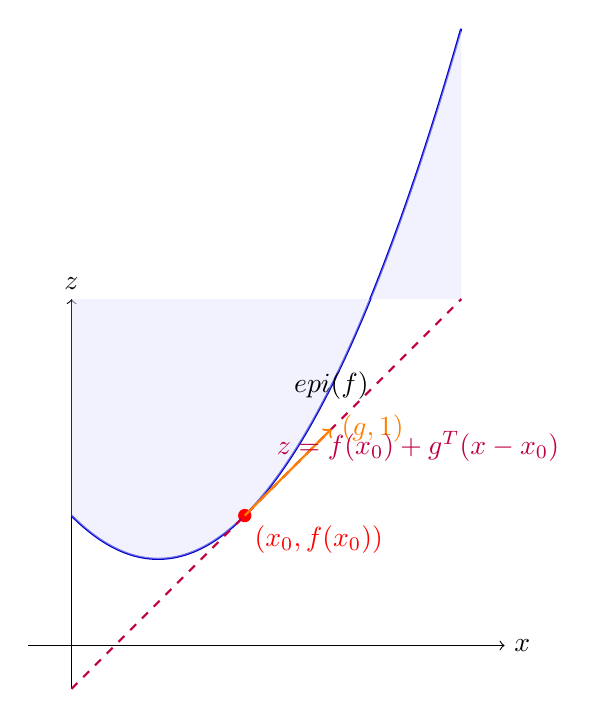
\begin{tikzpicture}[scale=1.1]
		% Koordinatsystem
		\draw[->] (-0.5,0) -- (5,0) node[right] {$x$};
		\draw[->] (0,-0.5) -- (0,4) node[above] {$z$};

		% Konveks funksjon
		\draw[thick, blue!80!black] plot [domain=0:4.5, samples=100] (\x, {0.5*\x*\x - 1*\x + 1.5});

		% Epigraf
		\fill[blue!10, opacity=0.5] (0,1.5) --
		plot [domain=0:4.5, samples=100] (\x, {0.5*\x*\x - 1*\x + 1.5}) --
		(4.5,4) -- (0,4) -- cycle;

		% Punkt på funksjonen
		\filldraw[red] (2,1.5) circle (2pt) node[below right] {$(x_0, f(x_0))$};

		% Subgradient/støttende hyperplan
		\draw[thick, purple, dashed] plot [domain=0:4.5, samples=2] (\x, {1.5 + 1*(\x-2)});

		% Vektor (subgradient)
		\draw[->, thick, orange] (2,1.5) -- (3,2.5) node[right] {$(g,1)$};

		\node at (3,3) {$\text{epi}(f)$};
		\node[purple] at (4,2.3) {$z = f(x_0) + g^T(x-x_0)$};
	\end{tikzpicture}
	\caption{Relasjonen mellom støttende hyperplan og subgradient. Hyperplanet $z = f(x_0) + g^T(x-x_0)$ støtter epigrafen til $f$ ved punktet $(x_0, f(x_0))$, hvor $g$ er en subgradient til $f$ ved $x_0$.}
	\label{fig:subgradient_supporting}
\end{figure}

\chapter{Konvekse Optimeringsproblemer}
\label{chap:convex_optimization}

\section{Problemformulering}
Vi vurderer optimaliseringsproblemer der vi minimerer en deriverbar funksjon \( f: \mathbb{R}^n \to \mathbb{R} \) over en konveks tillatt mengde \( \Omega \subseteq \mathbb{R}^n \):
\begin{mini*}
	{x \in \Omega}{f(x)}{}{}
\end{mini*}

Den tillatte mengden \( \Omega \) kan defineres på flere måter:
\begin{itemize}
	\item Eksplisitt som en konveks mengde, f.eks. \( \Omega = \{x : \|x\| \leq 1\} \)
	\item Gjennom likhetsbetingelser: \( \Omega = \{x : h(x) = 0\} \) der \( h \) er et system av affine funksjoner
	\item Gjennom ulikhetsbetingelser: \( \Omega = \{x : g(x) \leq 0\} \) der \( g \) er et system av konvekse funksjoner
	\item Kombinasjoner av de ovennevnte
\end{itemize}

\begin{definition}{Konvekst Optimeringsproblem}{convex_optimization_problem}
	Et konvekst optimeringsproblem har formen:
	\begin{mini*}
		{x \in \mathbb{R}^n}{f(x)}{}{}
		\addConstraint{g_i(x) \leq 0,}{i = 1, \ldots, m}
		\addConstraint{h_j(x) = 0,}{j = 1, \ldots, p}
	\end{mini*}
	hvor \( f \) og \( g_i \) er konvekse funksjoner, og \( h_j(x) = a_j^Tx - b_j \) er affine funksjoner.
\end{definition}

\begin{theorem}{Egenskaper ved Konveks Optimering}{convex_optimization_properties}
	For et konvekst optimeringsproblem:
	\begin{enumerate}
		\item Enhver lokal minimerer er en global minimerer.
		\item Mengden av minimerere, hvis ikke-tom, er konveks.
		\item Hvis \( f \) er strengt konveks, har problemet høyst én løsning.
		\item KKT-betingelsene er nødvendige og tilstrekkelige for optimalitet (under kvalifikasjonsbetingelser).
	\end{enumerate}
\end{theorem}

\section{Lineær Optimering (LP)}
Lineær optimering, eller lineær programmering, er en av de mest brukte optimeringsteknikkene i praksis. Vi vurderer problemer på formen:
\begin{mini*}
	{x\in\R^n}{c^Tx}{}{}
	\addConstraint{Ax}{\leq b}{}
	\addConstraint{Ex}{= d}{}
\end{mini*}
hvor \( A \in \R^{m \times n} \), \( E \in \R^{p \times n} \), \( c \in \R^n \), \( b \in \R^m \), og \( d \in \R^p \).

\subsection{Primal- og Dualproblemer i Lineær Programmering}
For hvert lineært programmeringsproblem (primalproblem) finnes det et tilhørende dualproblem:

\begin{maxi*}
	{y \in \R^m, z \in \R^p}{b^Ty + d^Tz}{}{}
	\addConstraint{A^Ty + E^Tz}{= c}{}
	\addConstraint{y}{\geq 0}{}
\end{maxi*}

Forholdet mellom primal- og dualproblemet gir verdifull innsikt:
\begin{itemize}
	\item Svak dualitet: Den optimale verdien av dualproblemet er alltid mindre enn eller lik den optimale verdien av primalproblemet.
	\item Sterk dualitet: Under milde betingelser er de optimale verdiene for primal- og dualproblemet like.
	\item Komplementær slakkhet: Hvis \( x^* \) og \( (y^*, z^*) \) er optimale løsninger for primal- og dualproblemet, gjelder \( y_i^*(A_ix^*-b_i) = 0 \) for alle \( i \).
\end{itemize}

\section{Kvadratisk Programmering (QP)}

\subsection{Kvadratiske Programmer med Likhetsbetingelser}
Kvadratiske programmer med kun likhetsbetingelser har formen:
\begin{mini*}
	{x\in\R^n}{\frac{1}{2}x^TQx + c^Tx}{}{}
	\addConstraint{Ax}{= b}{}
\end{mini*}
hvor \( Q \) er symmetrisk og positiv semidefinit.

For dette problemet gir KKT-betingelsene et system av lineære likninger:
\begin{align*}
	Qx + c + A^T\lambda & = 0 \\
	Ax                  & = b
\end{align*}

\subsection{Kvadratiske Programmer med Ulikhetsbetingelser}
Når ulikhetsbetingelser er til stede, blir problemet:
\begin{mini*}
	{x\in\R^n}{\frac{1}{2}x^TQx + c^Tx}{}{}
	\addConstraint{Ax}{\leq b}{}
	\addConstraint{Ex}{= d}{}
\end{mini*}

KKT-betingelsene inkluderer nå komplementær slakkhet:
\begin{align*}
	Qx + c + A^T\lambda + E^T\nu & = 0                 \\
	Ax                           & \leq b              \\
	Ex                           & = d                 \\
	\lambda                      & \geq 0              \\
	\lambda_i(A_ix - b_i)        & = 0 \quad \forall i
\end{align*}

\subsection{Aktiv Mengde-metoder}
Aktiv mengde-metoder løser kvadratiske programmeringsproblemer ved iterativt å oppdatere et estimat av den aktive mengden av betingelser ved løsningen. Hovedtrinnene er:

\begin{algorithm}[H]
	\caption{Aktiv Mengde-metode for QP}
	Finn et initialt tillatt punkt \( x_0 \)\;
	Identifiser de initialt aktive betingelsene \( \mathcal{A}_0 \)\;
	\For{\( k = 0, 1, 2, \ldots \)}{
		Løs QP med likhetsbetingelser ved å bruke betingelsene i \( \mathcal{A}_k \)\;
		Beregn Lagrange-multiplikatorene \( \lambda_i \) for aktive betingelser\;
		\eIf{alle \( \lambda_i \geq 0 \)}{
			Finn betingelsen med mest negativ \( \lambda_i \)\;
			Fjern denne betingelsen fra \( \mathcal{A}_k \)\;
		}{
			Finn stegretningsvektor \( p_k \)\;
			Beregn steglengde til nærmeste inaktive betingelse\;
			Oppdater \( x_{k+1} = x_k + \alpha_k p_k \)\;
			Oppdater \( \mathcal{A}_{k+1} \) med ny aktiv betingelse\;
		}
		\If{ingen betingelser å legge til eller fjerne}{
			\Return \( x_k \)\;
		}
	}
\end{algorithm}

\begin{definition}{Lineært optimeringsproblem}{linear_programming}
	Et lineært optimeringsproblem er et optimeringsproblem på formen
	\begin{mini*}
		{x\in\R^n}{c^Tx}{}{}
		\addConstraint{Ax}{\leq b,}{}
		\addConstraint{Dx}{= e,}{}
	\end{mini*}
	hvor \(c \in \R^n\) er en kostnadsvektor, \(A \in \R^{m \times n}\) er en matrise med ulikhetsbetingelser, \(D \in \R^{p \times n}\) er en matrise med likhetsbetingelser, og \(b \in \R^m\) og \(e \in \R^p\) er vektorer med høyre sideverdier.
\end{definition}

\begin{example}{Lineær funksjon}{linear_function}
	La \(f(\symbf{x}) = c^T\symbf{x} + d\) være en lineær funksjon, hvor \(c\) er en vektor normal til en hyperplan og \(d\) er en konstant.
	Da er \(f(\symbf{x}) = 0\) en lineær likning som definerer en hyperplan i \(\R^n\).
\end{example}

\begin{example}{Lineær regresjon}{linear_regression}
	La \(X \in \R^{n \times m}\) være en matrise med observasjoner og \(y \in \R^n\) være en vektor med målinger.
	Lineær regresjon er et eksempel på et lineært program hvor vi ønsker å finne en vektor \(w \in \R^m\) som minimerer kvadratfeilen
	\begin{equation*}
		\min_{w \in \R^m} \norm{Xw - y}_2^2.
	\end{equation*}
\end{example}

\chapter{Optimalitetsbetingelser}
\label{chap:optimality_conditions}

I konveks optimering spiller optimalitetsbetingelsene en avgjørende rolle for å karakterisere og finne optimale løsninger. Disse betingelsene gir oss teoretiske kriterier for å identifisere når et punkt er et minimum, og danner grunnlaget for effektive algoritmer.

\section{Førsteordens optimalitetsbetingelser}

Førsteordens betingelser bruker gradientinformasjon til å karakterisere optimale punkter. De er nødvendige for lokal optimalitet og ofte tilstrekkelige for global optimalitet når funksjonen er konveks.

\subsection{Gradient og retningsderiverte}

\begin{definition}{Gradient}{gradient}
	La $f: \mathbb{R}^n \to \mathbb{R}$ være en differensierbar funksjon. Gradienten til $f$ ved punktet $x$, betegnet $\nabla f(x)$, er vektoren av partielle deriverte:
	\[
		\nabla f(x) = \left(\frac{\partial f}{\partial x_1}, \frac{\partial f}{\partial x_2}, \ldots, \frac{\partial f}{\partial x_n}\right)^T
	\]
\end{definition}

Geometrisk representerer gradienten retningen av bratteste stigning for funksjonen ved punktet $x$. Den negative gradienten $-\nabla f(x)$ gir retningen av bratteste nedstigning, som er viktig for optimaliseringsalgoritmer.

For et ubetinget optimaliseringsproblem er en nødvendig førsteordens betingelse for at $x^*$ skal være et lokalt minimum:
\[
	\nabla f(x^*) = 0
\]

\subsection{Tillatte retninger}

Ved betingede optimaliseringsproblemer må vi vurdere om vi kan bevege oss i en gitt retning uten å bryte betingelsene.

\begin{definition}{Tillatte retninger}{feasible_directions}
	En vektor $d \in \mathbb{R}^n$ er en \textbf{tillatt retning} ved $x \in \Omega$ hvis det finnes en $\alpha > 0$ slik at $x + td \in \Omega$ for alle $t \in (0, \alpha]$.

	Mengden av alle tillatte retninger ved $x$ danner kjeglen av tillatte retninger, betegnet $\mathcal{F}_\Omega(x)$.
\end{definition}

\begin{definition}{Nedstigningsretning}{descent_direction}
	En retning $d \in \mathbb{R}^n$ er en \textbf{nedstigningsretning} for funksjonen $f$ ved $x$ hvis $\nabla f(x)^T d < 0$.
\end{definition}

For en optimal løsning $x^*$ finnes det ingen retning som både er tillatt og en nedstigningsretning.

\subsection{Nødvendige betingelser}

\begin{theorem}{Førsteordens nødvendige betingelse}{first_order_necessary}
	La $f: \mathbb{R}^n \to \mathbb{R}$ være en differensierbar funksjon og $\Omega \subset \mathbb{R}^n$ være en konveks mengde. Hvis $x^*$ er et lokalt minimum av $f$ over $\Omega$, da gjelder:
	\[
		\nabla f(x^*)^T (y - x^*) \geq 0 \quad \text{for alle } y \in \Omega
	\]
\end{theorem}

Denne betingelsen betyr at gradienten ved $x^*$ ikke peker i noen retning som ville føre til tillatte punkter med lavere funksjonsverdi. Den kan også uttrykkes som:
\[
	-\nabla f(x^*) \in N_\Omega(x^*)
\]
hvor $N_\Omega(x^*)$ er normalkjeglen til $\Omega$ ved $x^*$.

\begin{example}{Førsteordens betingelse}{first_order_example}
	For funksjonen $f(x) = x^2$ med $\Omega = \mathbb{R}$ er $x^* = 0$ et lokalt minimum. Her er $\nabla f(0) = 0$, så førsteordens betingelse er trivielt oppfylt.

	For funksjonen $f(x) = x$ med $\Omega = [0, \infty)$ er $x^* = 0$ et lokalt minimum. Her er $\nabla f(0) = 1$, og betingelsen verifiseres fordi:
	\[
		\nabla f(0)^T (y - 0) = y \geq 0 \quad \text{for alle } y \in [0, \infty)
	\]

	\begin{figure}[H]
		\centering
		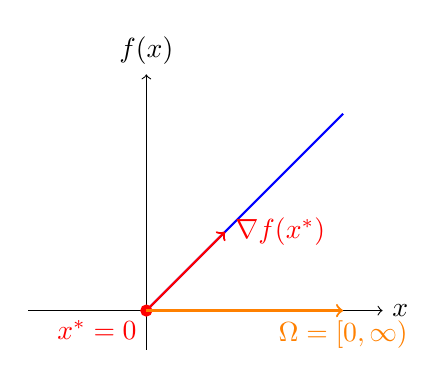
\begin{tikzpicture}
			% Axes
			\draw[->] (-1.5,0) -- (3,0) node[right] {$x$};
			\draw[->] (0,-0.5) -- (0,3) node[above] {$f(x)$};

			% Linear function
			\draw[thick, blue] (0,0) -- (2.5,2.5);

			% Point and gradient
			\filldraw[red] (0,0) circle (2pt) node[below left] {$x^*=0$};
			\draw[->, thick, red] (0,0) -- (1,1) node[right] {$\nabla f(x^*)$};

			% Feasible region
			\draw[thick, orange, ->] (0,0) -- (2.5,0) node[below] {$\Omega = [0,\infty)$};
		\end{tikzpicture}
		\caption{Førsteordens nødvendig betingelse for $f(x) = x$ med $\Omega = [0, \infty)$}
		\label{fig:first_order_example}
	\end{figure}
\end{example}

\subsection{Subgradienter for ikke-differensierbare funksjoner}

Når funksjonen ikke er differensierbar, generaliseres konseptet om gradient til subgradient.

\begin{definition}{Subgradient}{subgradient}
	En vektor $g \in \mathbb{R}^n$ er en \textbf{subgradient} av funksjonen $f$ ved et punkt $x$ hvis:
	\[
		f(y) \geq f(x) + g^T(y - x) \quad \text{for alle } y \in \mathbb{R}^n
	\]

	Mengden av alle subgradienter ved $x$ kalles \textbf{subdifferensialet} og betegnes $\partial f(x)$.
\end{definition}

For differensierbare funksjoner er subgradienten entydig og lik gradienten: $\partial f(x) = \{\nabla f(x)\}$.

\begin{example}{Subgradient av $l_1$-norm}{subgradient_l1}
	For funksjonen $f(x) = |x|$ (én-dimensjonal $l_1$-norm), er subdifferensialet ved $x$ gitt ved:
	\[
		\partial f(x) = \begin{cases}
			\{1\}   & \text{hvis } x > 0 \\
			\{-1\}  & \text{hvis } x < 0 \\
			[-1, 1] & \text{hvis } x = 0
		\end{cases}
	\]

	\begin{figure}[H]
		\centering
		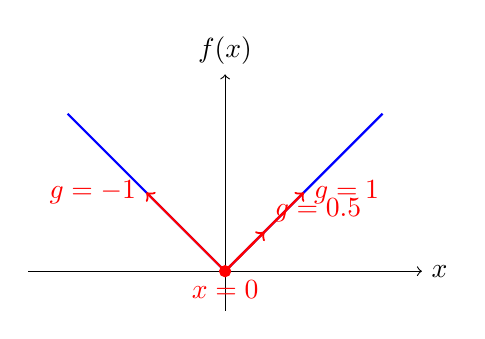
\begin{tikzpicture}
			% Axes
			\draw[->] (-2.5,0) -- (2.5,0) node[right] {$x$};
			\draw[->] (0,-0.5) -- (0,2.5) node[above] {$f(x)$};

			% Absolute value function
			\draw[thick, blue] (-2,2) -- (0,0) -- (2,2);

			% Point and subgradients
			\filldraw[red] (0,0) circle (2pt) node[below] {$x=0$};
			\draw[->, thick, red] (0,0) -- (1,1) node[right] {$g=1$};
			\draw[->, thick, red] (0,0) -- (-1,1) node[left] {$g=-1$};
			\draw[->, thick, red, dashed] (0,0) -- (0.5,0.5) node[above right] {$g=0.5$};
		\end{tikzpicture}
		\caption{Subgradienter av $f(x) = |x|$ ved $x = 0$}
		\label{fig:subgradient_l1}
	\end{figure}
\end{example}

Førsteordens nødvendige betingelse med subgradienter: Hvis $x^*$ er et lokalt minimum av $f$ over $\Omega$, da eksisterer det en subgradient $g \in \partial f(x^*)$ slik at:
\[
	g^T (y - x^*) \geq 0 \quad \text{for alle } y \in \Omega
\]

\section{Andreordens optimalitetsbetingelser}

Andreordens betingelser gir ytterligere informasjon om kurvingen til funksjonen ved et stasjonært punkt, og hjelper oss å skille mellom minimumspunkter, maksimumspunkter og sadelpunkter.

\subsection{Hessian}

\begin{definition}{Hessian}{hessian}
	Hessianen til en to ganger deriverbar funksjon $f: \mathbb{R}^n \to \mathbb{R}$ er matrisen av andrederiverte:
	\[
		\nabla^2 f(x) = H_f(x) = \begin{bmatrix}
			\frac{\partial^2 f}{\partial x_1^2}            & \frac{\partial^2 f}{\partial x_1 \partial x_2} & \cdots & \frac{\partial^2 f}{\partial x_1 \partial x_n} \\
			\frac{\partial^2 f}{\partial x_2 \partial x_1} & \frac{\partial^2 f}{\partial x_2^2}            & \cdots & \frac{\partial^2 f}{\partial x_2 \partial x_n} \\
			\vdots                                         & \vdots                                         & \ddots & \vdots                                         \\
			\frac{\partial^2 f}{\partial x_n \partial x_1} & \frac{\partial^2 f}{\partial x_n \partial x_2} & \cdots & \frac{\partial^2 f}{\partial x_n^2}
		\end{bmatrix}
	\]
\end{definition}

Hessianen beskriver den lokale krumningen av funksjonen. For en konveks funksjon er Hessianen positiv semidefinitt ved alle punkter.

\subsection{Andreordens betingelser}

\begin{theorem}{Andreordens nødvendige betingelse}{second_order_necessary}
	La $f: \mathbb{R}^n \to \mathbb{R}$ være en to ganger kontinuerlig deriverbar funksjon. Hvis $x^*$ er et lokalt minimum av $f$, da:
	\begin{itemize}
		\item $\nabla f(x^*) = 0$ (førsteordens betingelse)
		\item $\nabla^2 f(x^*) \succeq 0$ (Hessianen er positiv semidefinitt)
	\end{itemize}
\end{theorem}

\begin{theorem}{Andreordens tilstrekkelig betingelse}{second_order_sufficient}
	La $f: \mathbb{R}^n \to \mathbb{R}$ være en to ganger kontinuerlig deriverbar funksjon. Hvis:
	\begin{itemize}
		\item $\nabla f(x^*) = 0$
		\item $\nabla^2 f(x^*) \succ 0$ (Hessianen er positiv definitt)
	\end{itemize}
	da er $x^*$ et strengt lokalt minimum av $f$.
\end{theorem}

\subsection{Karakterisering av kritiske punkter}

For et kritisk punkt $x^*$ (der $\nabla f(x^*) = 0$) kan vi karakterisere dets type basert på Hessianen:

\begin{itemize}
	\item Hvis $\nabla^2 f(x^*) \succ 0$ (alle egenverdier positive): $x^*$ er et strengt lokalt minimum
	\item Hvis $\nabla^2 f(x^*) \prec 0$ (alle egenverdier negative): $x^*$ er et strengt lokalt maksimum
	\item Hvis $\nabla^2 f(x^*)$ har både positive og negative egenverdier: $x^*$ er et sadelpunkt
	\item Hvis $\nabla^2 f(x^*) \succeq 0$ med noen nullegenverdier: ytterligere analyse kreves
\end{itemize}

\begin{example}{Andreordens optimalisering}{second_order_example}
	Betrakt funksjonen $f(x,y) = x^2 + xy + y^2$. Vi kan finne kritiske punkter ved å løse:
	\begin{align}
		\nabla f(x,y) & = \begin{bmatrix} 2x + y \\ x + 2y \end{bmatrix} = \begin{bmatrix} 0 \\ 0 \end{bmatrix}
	\end{align}

	Dette gir $x = y = 0$ som eneste kritiske punkt. Hessianen er:
	\begin{align}
		\nabla^2 f(x,y) & = \begin{bmatrix} 2 & 1 \\ 1 & 2 \end{bmatrix}
	\end{align}

	Egenverdiene til denne matrisen er $\lambda_1 = 3$ og $\lambda_2 = 1$, som begge er positive. Dermed er $(0,0)$ et strengt lokalt minimum.

	\begin{figure}[H]
		\centering
		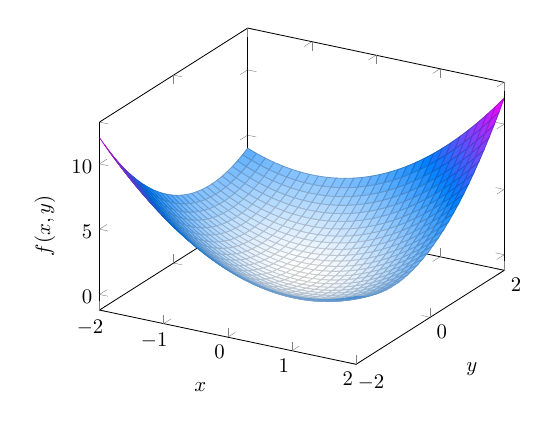
\begin{tikzpicture}[scale=0.75]
			\begin{axis}[
					xlabel={$x$},
					ylabel={$y$},
					zlabel={$f(x,y)$},
					view={30}{30},
					colormap/cool,
				]
				\addplot3[
					surf,
					domain=-2:2,
					domain y=-2:2,
					samples=30,
				]
				{x^2 + x*y + y^2};
			\end{axis}
		\end{tikzpicture}
		\caption{Grafen til funksjonen $f(x,y) = x^2 + xy + y^2$ med lokalt minimum ved $(0,0)$}
		\label{fig:second_order_example}
	\end{figure}
\end{example}

For betingede optimaliseringsproblemer utvides andreordens betingelser til å inkludere Lagrangefunksjonen og begrensingene, noe som fører til de mer generelle KKT-betingelsene.

\chapter{Dualitet}
\label{chap:duality}

For konvekse optimeringsproblemer kan vi definere et dualt problem som gir en nedre grense på verdien av det primale problemet. Under visse betingelser, som Slaters betingelse, vil det primale og duale problemet ha samme optimale verdi - dette kalles "sterk dualitet".

Dualitetsteori gir oss viktige innsikter om optimale løsninger og multiplikatorer, og danner grunnlaget for mange effektive algoritmer for konveks optimering.

\section{Lagrangian-funksjonen}

Lagrangian-funksjonen er et kraftfullt verktøy som omformer et betinget optimeringsproblem til et ubetinget problem. Den kombinerer målfunksjonen med begrensningene gjennom multiplikatorer, som vekter viktigheten av hver betingelse.

\begin{definition}{Lagrangian-funksjonen}{lagrangian}
	For det begrensede optimeringsproblemet:
	\begin{mini*}
		{x}{f(x)}{}{}
		\addConstraint{g_i(x)}{\leq 0,\quad}{i = 1, \ldots, m}
		\addConstraint{h_j(x)}{= 0,\quad}{j = 1, \ldots, p}
	\end{mini*}
	defineres Lagrangian-funksjonen som:
	\[
		\mathcal{L}(x, \lambda, \mu) = f(x) + \sum_{i=1}^m \lambda_i g_i(x) + \sum_{j=1}^p \mu_j h_j(x)
	\]
	hvor \( \lambda \in \mathbb{R}^m \) med \( \lambda \geq 0 \) er multiplikatorene for ulikhetsbegrensningene, og \( \mu \in \mathbb{R}^p \) er multiplikatorene for likhetsbegrensningene.
\end{definition}

For et mer generelt problem med både konkave ulikhetsbegrensninger og lineære likhetsbegrensninger kan Lagrangian-funksjonen uttrykkes som:
\begin{align*}
	\mathcal{L}(x, \lambda, \mu, v) & = f(x) - \sum_{i \in \mathcal{I}} \lambda_i c_i(x) - \langle\mu, Ax - b\rangle - \langle v, Cx - e\rangle
\end{align*}

hvor \(c_i(x)\) er konkave funksjoner, \(Ax \geq b\) representerer lineære ulikhetsbegrensninger, og \(Cx = e\) representerer lineære likhetsbegrensninger.

\paragraph{Betydning i optimeringsteori}
Lagrangian-funksjonen spiller en sentral rolle i begrenset optimering ved at:
\begin{itemize}
	\item Den danner grunnlaget for KKT-betingelsene, hvor \( \nabla_x \mathcal{L}(x, \lambda, \mu, v) = 0 \) er stasjonaritetsbetingelsen
	\item Den muliggjør formulering av dualproblemer gjennom den duale Lagrangian-funksjonen
	\item Sadelpunkter for Lagrangian-funksjonen korresponderer med optimale løsninger av det originale problemet
\end{itemize}

Ved å studere Lagrangian-funksjonen kan vi derfor få innsikt i både primal- og dualproblemet, samt karakterisere optimale løsninger.

\subsection{Svak og Sterk Dualitet}

\begin{definition}{Dualfunksjon}{dual_function}
	Dualfunksjonen \( g: \mathbb{R}^m \times \mathbb{R}^p \to \mathbb{R} \) er definert som:
	\[
		g(\lambda, \mu) = \inf_{x \in \mathbb{R}^n} \mathcal{L}(x, \lambda, \mu)
	\]
\end{definition}

\begin{definition}{Dualproblem}{dual_problem}
	Dualproblemet er:
	\begin{maxi*}
		{\lambda \geq 0, \mu}{g(\lambda, \mu)}{}{}
	\end{maxi*}
\end{definition}

\begin{theorem}{Svak Dualitet}{weak_duality}
	Hvis \( x \) er primal gjennomførbar og \( (\lambda, \mu) \) er dual gjennomførbare med \( \lambda \geq 0 \), da gjelder:
	\[
		g(\lambda, \mu) \leq f(x)
	\]
	Dette betyr at den optimale verdien for dualproblemet er en nedre grense for den optimale verdien for primalproblemet.
\end{theorem}

\begin{theorem}{Sterk Dualitet}{strong_duality}
	Hvis primalproblemet er konvekst og Slaters betingelse gjelder, da gjelder sterk dualitet: de optimale verdiene for primal- og dualproblemene er like.
\end{theorem}

\subsection{Sadelpunkter}

\begin{definition}{Sadelpunkt}{saddle_point}
	Et punkt \( (x^*, \lambda^*, \mu^*) \) er et sadelpunkt for Lagrange-funksjonen hvis:
	\[
		\mathcal{L}(x^*, \lambda, \mu) \leq \mathcal{L}(x^*, \lambda^*, \mu^*) \leq \mathcal{L}(x, \lambda^*, \mu^*)
	\]
	for alle \( x \in \mathbb{R}^n \), \( \lambda \geq 0 \), og \( \mu \in \mathbb{R}^p \).
\end{definition}

\begin{theorem}{Sadelpunktsetningen}{saddle_point_theorem}
	For et konvekst optimeringsproblem er \( (x^*, \lambda^*, \mu^*) \) et sadelpunkt for Lagrange-funksjonen hvis og bare hvis:
	\begin{itemize}
		\item \( x^* \) er primal optimalt
		\item \( (\lambda^*, \mu^*) \) er dual optimalt
		\item Sterk dualitet gjelder
	\end{itemize}
\end{theorem}

\subsection{Lagrangedualitet}

Lagrangedualitet gir en systematisk måte å utlede dualproblemer og etablere dualitetsresultater.

\begin{theorem}{Lagrangedualitet}{lagrangian_duality}
	For et konvekst optimeringsproblem:
	\[
		\min_{x \in \mathbb{R}^n} f(x) = \min_{x \in \mathbb{R}^n} \max_{\lambda \geq 0, \mu} \mathcal{L}(x, \lambda, \mu)
	\]
	Når sterk dualitet gjelder:
	\[
		\min_{x \in \mathbb{R}^n} \max_{\lambda \geq 0, \mu} \mathcal{L}(x, \lambda, \mu) = \max_{\lambda \geq 0, \mu} \min_{x \in \mathbb{R}^n} \mathcal{L}(x, \lambda, \mu)
	\]
\end{theorem}

\subsection{Legendre-Fenchel-transformasjonen}

\begin{definition}{Legendre-Fenchel-transformasjonen}{legendre_fenchel}
	Legendre-Fenchel-transformasjonen (eller konveks konjugasjon) av en funksjon \( f: \mathbb{R}^n \to \mathbb{R} \cup \{+\infty\} \) er:
	\[
		f^*(y) = \sup_{x \in \mathbb{R}^n} \{y^Tx - f(x)\}
	\]
\end{definition}

\begin{theorem}{Egenskaper ved Legendre-Fenchel-transformasjonen}{legendre_fenchel_properties}
	Legendre-Fenchel-transformasjonen har flere viktige egenskaper:
	\begin{itemize}
		\item \( f^* \) er alltid konveks, selv om \( f \) ikke er det
		\item Hvis \( f \) er konveks og nedre halvkontinuerlig, da gjelder \( (f^*)^* = f \)
		\item Hvis \( f \) er strengt konveks og deriverbar, da gjelder \( \nabla f^*(y) = x \) der \( y = \nabla f(x) \)
	\end{itemize}
\end{theorem}

Legendre-Fenchel-transformasjonen gir kraftige verktøy for dualitetsteori og konveks analyse, og kobler problemer gjennom deres duale formuleringer.

\section{Betingelseskvalifikasjoner}

For å sikre at optimalitetsbetingelsene er gyldige og at vi kan finne Lagrange-multiplikatorer, trenger vi visse betingelser kjent som \enquote{Constraint Qualifications} (CQ).
Disse betingelsene sikrer at de aktive betingelsene er lineært uavhengige og at det ikke er noen redundante betingelser.

Noen vanlige betingelseskvalifikasjoner er:
\begin{itemize}
	\item Slaters betingelse (Slater's condition)
	\item Linear Independence Constraint Qualification (LICQ)
	\item Manglende komplementaritet (MFCQ)
	\item Manglende aktiv mengde (MFCQ)
\end{itemize}

\subsection{Slaters betingelse}
\label{sec:slater_condition}

Slaters kvalifikasjon for begrensninger er en viktig betingelse i konveks optimering som sikrer sterk dualitet og gyldigheten av KKT-betingelsene.

\begin{definition}{Slaters betingelse}{slater_condition}
	For et konvekst optimeringsproblem:
	\begin{mini*}
		{x}{f(x)}{}{}
		\addConstraint{g_i(x)}{\leq 0,\quad}{i = 1, \ldots, m}
		\addConstraint{Ax}{= b}{}
	\end{mini*}
	der \( f \) og \( g_i \) er konvekse, gjelder Slaters betingelse hvis det finnes et punkt \( \bar{x} \) slik at:
	\begin{itemize}
		\item \( g_i(\bar{x}) < 0 \) for alle \( i = 1, \ldots, m \) (strikt ulikhet)
		\item \( A\bar{x} = b \)
	\end{itemize}
	Dette punktet \( \bar{x} \) kalles et strengt gjennomførbart punkt.
\end{definition}

\begin{remark}{Intuisjon}{slater_intuition}
	Slaters betingelse garanterer at det tillatte området har et ikke-tomt indre med hensyn til ulikhetsbetingelsene.
	Med andre ord: betingelsene er ikke alle \enquote{stramme} i hvert punkt, noe som sikrer at det finnes en viss \enquote{frihet} i det tillatte området.

	Det er viktig for å etablere sterk dualitet, og at det eksisterer Lagrange-multiplikatorer som oppfyller KKT-betingelsene.
\end{remark}

\begin{theorem}{Viktigheten av Slaters Betingelse}{slater_importance}
	For et konvekst optimeringsproblem som tilfredsstiller Slaters betingelse:
	\begin{enumerate}
		\item Sterk dualitet gjelder: de optimale verdiene for primal- og dualproblemene er like
		\item Hvis den optimale verdien for primalproblemet er endelig, oppnås den optimale verdien for dualproblemet
		\item KKT-betingelsene er både nødvendige og tilstrekkelige for global optimalitet
	\end{enumerate}
\end{theorem}

\subsection{LICQ (Linear Independence Constraint Qualification)}
\label{sec:LICQ}

Et ikke-lineært optimeringsproblem kan skrives på følgende form:
\begin{mini*}
	{x \in \mathbb{R}^n}{f(x)}{}{}
	\addConstraint{c_i(x)}{= 0,\quad}{ i \in \mathcal{E}}
	\addConstraint{c_j(x)}{\leq 0,\quad}{ j \in \mathcal{I}}
\end{mini*}

Her er \(f : \mathbb{R}^n \to \mathbb{R}\) objektivfunksjonen, mens \(c_i(x)\) og \(c_j(x)\) representerer henholdsvis likhets- og ulikhetsbetingelsene som definerer løsningsrommet \(\Omega\).

For å sikre at standard optimalitetsbetingelser gjelder, trenger vi kvalifikasjonsbetingelser for løsningsrommet. LICQ er en av de viktigste slike betingelsene.

\begin{definition}{Linear Independence Constraint Qualification (LICQ)}{licq}
	La \( x^* \) være et tillatt punkt. Vi definerer mengden av aktive betingelser ved \(x^*\) som:
	\[
		\mathcal{A}(x^*) = \{ i \in \mathcal{E} \cup \mathcal{I} \mid c_i(x^*) = 0 \}.
	\]
	LICQ er oppfylt ved \( x^* \) hvis gradientene til alle aktive betingelser
	\[
		\{\nabla c_i(x^*) : i \in \mathcal{A}(x^*)\}
	\]
	er lineært uavhengige i \( \mathbb{R}^n \). Dette betyr formelt at:
	\[
		\sum_{i \in \mathcal{A}(x^*)} \lambda_i \nabla c_i(x^*) = 0
		\quad \Longrightarrow \quad
		\lambda_i = 0 \;\text{for alle}\; i \in \mathcal{A}(x^*).
	\]
\end{definition}

\begin{remark}{Betydning av LICQ}{}
	LICQ er avgjørende i optimeringsteori av flere grunner:
	\begin{itemize}
		\item \textbf{Eksistens av Lagrange-multiplikatorer:} Hvis \(x^*\) er et lokalt minimum og LICQ gjelder,
		      eksisterer en unik vektor \(\lambda^*\) av multiplikatorer slik at KKT-betingelsene oppfylles:
		      \[
			      \nabla f(x^*) = \sum_{i \in \mathcal{A}(x^*)}\lambda_i^*\nabla c_i(x^*),\quad
			      \lambda_j^* \geq 0 \text{ for aktive ulikheter}
		      \]

		\item \textbf{Lokal regularitet:} LICQ sikrer at Jakobi-matrisen for de aktive betingelsene har full rang,
		      hvilket er nødvendig for anvendelsen av KKT-betingelser.

		\item \textbf{Unikhet:} Når LICQ er oppfylt, er Lagrange-multiplikatorene entydige, slik at KKT-systemet
		      har en unik løsning.
	\end{itemize}

	Hvis LICQ ikke holder, kan det oppstå vanskeligheter med å finne Lagrange-multiplikatorene,
	og KKT-betingelsene kan bli ugyldige eller gi flere løsninger.
\end{remark}

\subsubsection{Normalkjeglen}
Under forutsetning av LICQ (Linear Independence Constraint Qualification) kan normalkjeglen uttrykkes som:
\begin{equation*}
	N_{\Omega}(x) = \left\{\sum_{i \in I(x)} \lambda_i \nabla g_i(x) + \sum_{j=1}^p \mu_j \nabla h_j(x) \mid \lambda_i \geq 0 \right\},
\end{equation*}
hvor \(I(x) = \{i \mid g_i(x) = 0\}\) er indeksen til de aktive ulikhetsbetingelsene.


\begin{example}{LICQ med flere ulikhetsbetingelser}{}
	Betrakt følgende optimeringsproblem:
	\begin{mini*}
		{x,y}{(x-1)^2 + (y+2)^2}{}{}
		\addConstraint{c_1(x,y) &= -x}{\leq 0}{}
		\addConstraint{c_2(x,y) &= x-2-y}{\leq 0}{}
		\addConstraint{c_3(x,y) &= 1-(x-1)^2-y^2}{\leq 0}{}
	\end{mini*}

	Ved et punkt \(P\) hvor alle tre betingelser er aktive, har vi følgende gradienter:
	\begin{align*}
		\nabla c_1(x,y) & = (-1,0),        \\
		\nabla c_2(x,y) & = (1,-1),        \\
		\nabla c_3(x,y) & = (-2(x-1),-2y).
	\end{align*}

	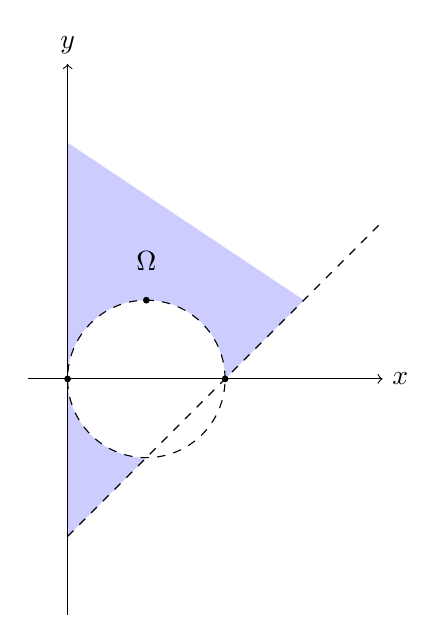
\begin{tikzpicture}
		% Feasible region 
		\fill[blue!20] (0, -2) -- (0, 3) -- (3, 1) -- cycle;
		\fill[white] (1, 0) circle(1cm);

		\filldraw[black] (1,1) circle (1pt);
		\filldraw[black] (2,0) circle (1pt);
		\filldraw[black] (0,0) circle (1pt);

		\draw[->] (-0.5, 0) -- (4, 0) node[right] {\(x\)};
		\draw[->] (0, -3) -- (0, 4) node[above] {\(y\)};

		% Draw constraints
		\draw[dashed] (1, 0) circle(1cm);
		\draw[dashed] (0, -2) -- (4, 2);
		\draw[dashed] (0, -2) -- (0, 3);

		\node at (1, 1.5) {\(\Omega\)};
	\end{tikzpicture}

	Ved punkt \(P\) hvor alle betingelser møtes, peker gradientene i forskjellige retninger og er lineært uavhengige.
	Derfor er LICQ oppfylt ved dette punktet, hvilket muliggjør bruk av KKT-betingelsene for å finne den optimale løsningen.
\end{example}

\begin{remark}{LICQ -- Sammendrag}{}
	LICQ sikrer at gradientene til de aktive betingelsene ved et punkt \(x^*\) er lineært uavhengige. Vi husker:

	\paragraph{Aktive betingelser} En betingelse er aktiv hvis:
	\[ \begin{cases}
			c_i(x) = 0 & \text{for likhetsbetingelser}  \\
			c_j(x) = 0 & \text{for ulikhetsbetingelser}
		\end{cases} \]

	\paragraph{Lineær uavhengighet} Gradientene \(\{\nabla c_k(x^*)\}\) er lineært uavhengige når:
	\[
		\sum_k \alpha_k \nabla c_k(x^*) = 0 \implies \alpha_k = 0 \text{ for alle } k
	\]

	Dette er avgjørende for eksistensen av Lagrange-multiplikatorene og anvendelsen av KKT-betingelsene.
\end{remark}

\subsection{Farkas' Lemma}

Farkas' lemma er et grunnleggende resultat innen konveks analyse og optimering som karakteriserer når en lineær ulikhet er en konsekvens av et system av lineære ulikheter.

\begin{lemma}{Farkas' Lemma}{farkas_lemma}
	La \( A \in \mathbb{R}^{m \times n} \) og \( c \in \mathbb{R}^n \). Da er nøyaktig én av følgende to utsagn sanne:
	\begin{enumerate}
		\item Det finnes en \( x \in \mathbb{R}^n \) slik at \( Ax \leq 0 \) og \( c^Tx > 0 \).
		\item Det finnes en \( y \in \mathbb{R}^m \) slik at \( y \geq 0 \) og \( A^Ty = c \).
	\end{enumerate}
\end{lemma}

\begin{lemma}{Farka's Lemma}{farkas_lemma}
	Let \(A \in \mathbb{R}^{m \times n}\) and \(c \in \mathbb{R}^n\). Then, exactly one of the following statements is true:
	\begin{enumerate}
		\item[] \((1)\) There exists an \(x \in \mathbb{R}^n\) such that \(Ax \preceq 0\) and \(c^T x < 0\).
		\item[] \((2)\) There exists a \(y \in \mathbb{R}^m\) such that \(A^T y + c = 0\) and \(y \succeq 0\).
	\end{enumerate}
\end{lemma}

Farkas' lemma brukes ofte til å etablere eksistensen av Lagrange-multiplikatorer og til å utlede dualitetsresultater i optimering.

\begin{proof}
	\begin{enumerate}
		\item[] Assume that \((1)\) holds. Then \(Ax = b\) and \(x \ge 0\). If there exists a \(y\) such that \(y^T A \ge 0\), then
		      \[
			      y^T b = y^T Ax = (y^T A)x \ge 0,
		      \]
		      which contradicts \(y^T b < 0\).
		\item[] Assume that \((1)\) does not hold. We want to show that \((2)\) holds.

		      Let
		      \[
			      K = \{Ax \mid x \ge 0\}.
		      \]
		      Since \((1)\) does not hold, \(b \notin K\). Since \(K\) is a closed convex cone, by the separating hyperplane theorem, there exists a \(y \in \mathbb{R}^m\) such that
		      \[
			      y^T b < y^T z \quad \text{for all } z \in K.
		      \]
		      Since \(0 \in K\), we have \(y^T b < 0\).

		      Now, for any \(x \ge 0\), we have \(Ax \in K\), so \(y^T b < y^T Ax\).

		      Let \(x = e_i\), where \(e_i\) is the \(i\)-th standard basis vector. Then \(x \ge 0\), and
		      \[
			      y^T A e_i = (y^T A)_i > 0.
		      \]
		      Thus \(y^T A \ge 0\).
	\end{enumerate}

	\begin{center}
		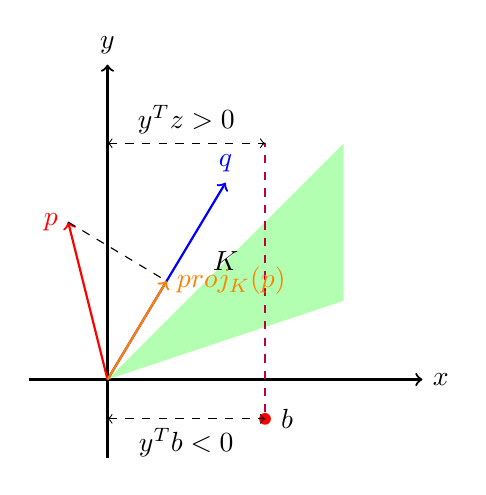
\begin{tikzpicture}
			\draw[->, thick] (-1, 0) -- (4, 0) node[right] {\( x \)};
			\draw[->, thick] (0, -1) -- (0, 4) node[above] {\( y \)};

			\fill[green!30] (0, 0) -- (3, 1) -- (3, 3) -- cycle;
			\node at (1.5, 1.5) {\( K \)};

			\node[circle, fill=red, inner sep=1.5pt, label=right:\( b \)] (b) at (2, -0.5) {};

			\draw[dashed, purple] (b) -- (2, 3);
			\draw[<->, dashed, black] (0, -0.5) -- (2, -0.5) node[midway, below, black] {\( y^Tb < 0 \)};
			\draw[<->, dashed, black] (0, 3) -- (2, 3) node[midway, above, black] {\( y^Tz > 0 \)};

			% Adding new vectors
			\draw[->, thick, blue] (0, 0) -- (1.5, 2.5) node[above] {\( q \)};
			\draw[->, thick, red] (0, 0) -- (-0.5, 2) node[left] {\( p \)};
			\draw[->, thick, orange] (0, 0) -- (0.75, 1.25) node[right] {\( proj_K(p) \)};
			\draw[dashed] (-0.5, 2) -- (0.75, 1.25);
		\end{tikzpicture}
	\end{center}

	The figure illustrates the geometric interpretation of Farkas' Lemma. The green region \( K \) represents the cone of feasible points \( \{Ax \mid x \ge 0\} \). The point \( b \) (in red) lies outside this cone. The purple dashed line represents the separating hyperplane, which separates \( b \) from \( K \). Vector \( p \) (in red) is projected onto the cone \( K \), resulting in \( proj_K(p) \) (in orange). Vector \( q \) (in blue) lies inside the cone \( K \). The black dashed lines show that the inner product \( y^Tb \) is negative, while the inner product \( y^Tz \) is positive for points \( z \) in the cone \( K \).
\end{proof}

\section{KKT-betingelsene}
\label{sec:kkt_conditions}
\begin{center}
	\begin{tikzpicture}[
			node distance=0.8cm and 0.8cm,
			every node/.style={draw, rectangle, rounded corners=3pt, align=center, font=\sffamily\scriptsize},
			>=stealth, thick,
			startstop/.style={rectangle, rounded corners, draw, fill=cor-color!15, text width=9em, minimum height=1em},
			block/.style={rectangle, draw, fill=thm-color!10, text width=10em, rounded corners, minimum height=1em},
			decision/.style={diamond, draw, fill=lem-color!10, text width=5em, text badly centered, inner sep=0pt, aspect=1.5}
		]

		% Top-level problem
		\node [startstop] (start) {
			\textbf{Betinget Optimeringsproblem}\\[0.5ex]
			Minimer \( f(x) \) gitt\\
			\( c_i(x)=0,\;i\in E \);\\
			\( c_j(x)\ge0,\;j\in I \)
		};

		% Decision: convex?
		\node [decision, below=1.0cm of start] (convexq) {
			Er problemet\\
			\emph{konvekst}?
		};

		% --- Convex branch (left) ---
		\node [block, below left=1.0cm and 2cm of convexq] (slater) {
			\textbf{Sjekk Slaters Betingelse}\\[0.5ex]
			(for konvekse problemer)\\
			Sikrer sterk dualitet \& KKT gyldighet
		};

		\node [decision, below=1.0cm of slater] (cqok2) {
			Slater\\oppfylt?
		};

		\node [block, below=1.0cm of cqok2] (cqsat2) {
			\textbf{Slater's Betingelse:}\\[0.5ex]
			Eksisterer et punkt \( \bar{x} \) der\\
			\( c_j(\bar{x}) > 0 \) for \( j \in I \),\\
			\( c_i(\bar{x}) = 0 \) for \( i \in E \),\\
			og \( c_j(\bar{x}) \) er \emph{strikt} positiv
		};

		% --- Nonconvex branch (right) ---
		\node [block, below right=1.0cm and 2cm of convexq] (licq) {
			\textbf{Sjekk KK for ikke-konvekse:}\\[0.5ex]
			\textbf{LICQ} eller MFCQ, osv.\\
			Hvis ikke oppfylt, KKT gjelder kanskje ikke
		};

		\node [decision, below=1.0cm of licq] (cqok) {
			KK\\oppfylt?
		};

		\node [block, below=1.0cm of cqok] (cqsat) {
			\textbf{LICQ:}\\[0.5ex]
			Eksisterer et punkt \( \bar{x} \) der\\
			\( c_i(\bar{x}) = 0 \) for \( i \in E \)\\
			\( c_j(\bar{x}) > 0 \) for \( j \in I \),\\
			og \( \nabla c_i(\bar{x}) \) er lineært uavhengige
		};

		% Failure node (shared by both branches)
		\node [block, below=1.0cm of convexq] (fail) {
			\textbf{Ingen KK oppfylt:}\\[0.5ex]
			KKT kan feile\\
			Bruk alternative metoder
		};

		% --- Common branch: KKT, Second-order, Conclusion ---
		\node [block, below=3.5cm of convexq] (kkt) {
			\textbf{KKT-betingelser:}\\[0.5ex]
			1. Stasjonaritet: \( \nabla f(x^*) + \sum_i \lambda_i \nabla c_i(x^*) = 0 \)\\
			2. Primal gyldighet: \( c_i(x^*) = 0 \) eller \( c_j(x^*) \geq 0 \)\\
			3. Dual gyldighet: \( \lambda_j \geq 0 \) for \( j \in I \)\\
			4. Komplementær slakkhet: \( \lambda_j\,c_j(x^*) = 0 \)
		};

		\node [block, below=1.0cm of kkt] (second) {
			\textbf{Andregrads-betingelser:}\\[0.5ex]
			\emph{Nødvendig:} \( \nabla_{xx}^2 \mathcal{L}(x^*,\lambda^*) \succeq 0 \)\\[0.5ex]
			\emph{Tilstrekkelig:} \( \nabla_{xx}^2 \mathcal{L}(x^*,\lambda^*) \succ 0 \)
		};

		\node [startstop, below=1.0cm of second] (conclude) {
			\textbf{Konklusjon}\\[0.5ex]
			Hvis KKT + 2.-grads betingelser holder,\\
			\( \;x^* \) er lokalt minimum.\\[0.5ex]
			Under konveksitet er \( \;x^* \) globalt minimum.
		};

		% -----------------
		% Connections
		\draw [->, thick] (start) -- (convexq);
		\draw [->, thick] (convexq) -- node[above left, font=\tiny, fill=white] {Yes} (slater);
		\draw [->, thick] (convexq) -- node[above right, font=\tiny, fill=white] {No} (licq);

		% Convex branch
		\draw [->, thick] (slater) -- (cqok2);
		\draw [->, thick] (cqok2) -- node[font=\tiny, fill=white] {Yes} (cqsat2);
		\draw [->, thick] (cqok2.east) -- ++(1,0) |- node[font=\tiny, fill=white] {No} (fail.west);
		\draw [->, thick] (cqsat2.east) -- ++(0.5,0) |- (kkt.west);

		% Nonconvex branch
		\draw [->, thick] (licq) -- (cqok);
		\draw [->, thick] (cqok) -- node[font=\tiny, fill=white] {Yes} (cqsat);
		\draw [->, thick] (cqok.west) -- ++(-1,0) |- node[font=\tiny, fill=white] {No} (fail.east);
		\draw [->, thick] (cqsat.west) -- ++(-0.5,0) |- (kkt.east);

		% Common branch
		\draw [->, thick] (kkt) -- (second);
		\draw [->, thick] (second) -- (conclude);
	\end{tikzpicture}
\end{center}

Karush-Kuhn-Tucker (KKT)-betingelsene er sentrale i konveks optimering og gir nødvendige og tilstrekkelige betingelser for optimalitet når visse kvalifikasjonsbetingelser er oppfylt.

\subsection{Generell Formulering}

\begin{theorem}{KKT-betingelser}{kkt_conditions}
	La oss betrakte optimeringsproblemer på formen:
	\begin{mini*}
		{x}{f(x)}{}{}
		\addConstraint{g_i(x)}{\leq 0,\quad}{i = 1, \ldots, m}
		\addConstraint{h_j(x)}{= 0,\quad}{j = 1, \ldots, p}
	\end{mini*}

	Hvis $x^*$ er et lokalt minimum og en passende kvalifikasjonsbetingelse (som LICQ eller Slaters betingelse) er oppfylt, så finnes det Lagrange-multiplikatorer $\lambda^* \in \mathbb{R}^m$ og $\mu^* \in \mathbb{R}^p$ slik at følgende betingelser er oppfylt:

	\begin{align}
		\nabla f(x^*) + \sum_{i=1}^m \lambda_i^* \nabla g_i(x^*) + \sum_{j=1}^p \mu_j^* \nabla h_j(x^*) & = 0 \tag{Stasjonaritet}                                              \\
		g_i(x^*)                                                                                        & \leq 0, \quad \forall i = 1, \ldots, m \tag{Primal gjennomførbarhet} \\
		h_j(x^*)                                                                                        & = 0, \quad \forall j = 1, \ldots, p \tag{Primal gjennomførbarhet}    \\
		\lambda_i^*                                                                                     & \geq 0, \quad \forall i = 1, \ldots, m \tag{Dual gjennomførbarhet}   \\
		\lambda_i^* g_i(x^*)                                                                            & = 0, \quad \forall i = 1, \ldots, m \tag{Komplementær slakkhet}
	\end{align}
\end{theorem}


\begin{itemize}
	\item \textbf{Stasjonaritetsbetingelsen:} Gradienten til målfunksjonen må kunne uttrykkes som en lineær kombinasjon av gradientene til aktive begrensninger ved den optimale løsningen.

	\item \textbf{Primal gjennomførbarhet:} Løsningen må tilfredsstille alle opprinnelige begrensninger i optimeringsproblemer.

	\item \textbf{Dual gjennomførbarhet:} Lagrange-multiplikatorene for ulikhetsbegrensninger må være ikke-negative.

	\item \textbf{Komplementær slakkhet:} For hver ulikhetsbegrensning må enten begrensningen være aktiv ($g_i(x^*) = 0$) eller den tilhørende multiplikatoren må være null ($\lambda_i^* = 0$).
\end{itemize}

\subsection{KKT-betingelser for konvekse problemer}

For konvekse optimeringsproblemer, der $f$ og $g_i$ er konvekse funksjoner og $h_j$ er affine funksjoner, gjelder:

\begin{theorem}{KKT-betingelser for Konvekse Problemer}{kkt_convex}
	Hvis Slaters betingelse er oppfylt for et konvekst optimeringsproblem, er KKT-betingelsene både nødvendige og tilstrekkelige for global optimalitet.
	Det vil si at $x^*$ er en global løsning hvis og bare hvis det eksisterer multiplikatorer $\lambda^*$ og $\mu^*$ som sammen med $x^*$ oppfyller KKT-betingelsene.
\end{theorem}

\begin{proof}{KKT-betingelser for konvekse problemer}{}
	We have the optimality condition:
	\[
		\inner{\nabla f(x^\star), p} \geq 0 \, \forall p \in T_{\Omega}(x^\star)
	\]
	\medskip
	\begin{align*}
		p \in T_{\Omega}(x^\star) \iff
		\begin{cases}
			\inner{\nabla c_i (x^\star), p }\geq 0                             & \forall i \in \mathcal{A}_1(x^\star) \\
			\text{or: there does not exist any } p \in \R^d \text{ such that:} &                                      \\
			\begin{cases}
				\inner{\nabla c_i (x^\star), p }\geq 0 & \forall i \in \mathcal{A}_1(x^\star) \\
				\inner{A_i^T , p }\geq 0               & \forall i \in \mathcal{A}_2(x^\star) \\
				\inner{ (C_i )^T, p } = 0              & \forall 1 \leq i \leq l              \\
				\inner{\nabla f (x^\star), p } < 0     &
			\end{cases}                             \\
			(Ap)_i \geq 0                                                      & \forall i \in \mathcal{A}_2(x^\star) \\
			Cp = 0                                                             &
		\end{cases}
	\end{align*}

	The second alternative is Farka's Lemma does not hold \(\implies\) The first holds.

	\begin{align*}
		\nabla f(x^\star) & = \sum_{i\in \mathcal{A}_1(x^\star)} \lambda_i^\star \nabla c_i(x^\star) + \sum_{i \in \mathcal{A}_2(x^\star)} \mu_i^\star A_i^T + \sum_{i=1}^l v_i^\star C_i^T \\
	\end{align*}

	For some  \(\lambda_i^\star \geq 0, \mu_i^\star \geq 0, v_i^\star \in \R\).

	Now define: \(\lambda_i^\star = 0 \) for \(i \notin \mathcal{A}_1(x^\star)\) and \(\mu_i^\star = 0\) for \(i \notin \mathcal{A}_2(x^\star)\).

	Then we have:
	\begin{align*}
		\nabla f(x^\star) & = \sum_{i\in \mathcal{I}} \lambda_i^\star \nabla c_i(x^\star) + \sum_{1 \leq i \leq m} \mu_i^\star A_i^T + \sum_{1 \leq i \leq l} v_i^\star C_i^T = \text{(1)} \\
	\end{align*}
	\qed
\end{proof}

\subsection{Aktive Begrensninger og Tangentkjegle}

Vi definerer aktive begrensninger ved et punkt $x$ som:
\begin{align*}
	\mathcal{A}(x) = \{i \in \{1,\ldots,m\} \mid g_i(x) = 0\} \cup \{j+m \in \{m+1,\ldots,m+p\} \mid h_j(x) = 0\}
\end{align*}

Tangentkjeglen ved et tillatt punkt $x$ kan karakteriseres som:
\begin{align*}
	p \in T_{\Omega}(x) \Longleftrightarrow
	\begin{cases}
		\langle \nabla g_i(x), p \rangle \leq 0, & \forall i \in \mathcal{A}(x) \cap \{1,\ldots,m\} \\
		\langle \nabla h_j(x), p \rangle = 0,    & \forall j \in \{1,\ldots,p\}
	\end{cases}
\end{align*}

Dette betyr at en retning er tillatt hvis den respekterer både aktive ulikhetsbegrensninger og alle likhetsbegrensninger.

\begin{remark}{Geometrisk Tolkning av KKT-betingelsene}{}
	KKT-betingelsene har en klar geometrisk tolkning som er nyttig for å forstå deres betydning:

	\begin{itemize}
		\item \textbf{Stasjonæritetsbetingelsen:} Gradienten til målfunksjonen kan uttrykkes som en lineær kombinasjon av gradientene til de aktive betingelsene. Dette betyr at det ikke finnes noen tillatt retning som reduserer målfunksjonen.

		\item \textbf{Primal gjennomførbarhet:} Sikrer at løsningen tilfredsstiller alle opprinnelige betingelser i optimeringsproblemer.

		\item \textbf{Dual gjennomførbarhet:} Multiplikatorene for ulikheter er ikke-negative, som sikrer at vi beveger oss i riktig retning langs betingelsene.

		\item \textbf{Komplementær slakkhet:} En betingelse må enten være aktiv ($g_i(x^*) = 0$), eller så må den tilhørende multiplikatoren være null ($\lambda_i^* = 0$). Dette betyr at vi bare tar hensyn til aktive begrensninger; inaktive begrensninger har ingen påvirkning på optimaliteten.

		\item Hvis $\lambda_i^* > 0$ for en aktiv begrensning, indikerer dette at å relaksere denne begrensningen vil forbedre den optimale verdien. $\lambda_i^*$ tolkes ofte som skyggeprisen eller sensitiviteten til den optimale verdien med hensyn til endringer i begrensning $i$.
	\end{itemize}
\end{remark}

\chapter{Metoder}
\label{sec:convex_optimization_methods}

\section{Projeksjoner på Konvekse Mengder}
For et hvilket som helst punkt \( x \in \mathbb{R}^n \) og en lukket konveks mengde \( \Omega \), er projeksjonen av \( x \) på \( \Omega \) definert som:
\[
	P_\Omega(x) = \arg\min_{y \in \Omega} \|y - x\|_2
\]

\subsection{Egenskaper til Projeksjoner}
\begin{itemize}
	\item Projeksjonen på en lukket konveks mengde eksisterer alltid og er unik.
	\item \( x = P_\Omega(x) \) hvis og bare hvis \( x \in \Omega \).
	\item Geometrisk karakterisering: \( P_\Omega(x) \) er det unike punktet \( y \in \Omega \) slik at \( (x - y)^T(z - y) \leq 0 \) for alle \( z \in \Omega \).
\end{itemize}

\subsection{Projisert Gradientmetode}
En naturlig utvidelse av gradientmetoden for optimalisering med begrensninger er den projiserte gradientmetoden:
\[
	x_{k+1} = P_\Omega(x_k - \alpha_k \nabla f(x_k))
\]
der \( \alpha_k \) er steglengden.

Den projiserte gradientmetoden har konvergensgarantier som ligner på gradientmetoden når den brukes på konvekse funksjoner og konvekse tillatte mengder.

\begin{algorithm}[H]
	\caption{Projisert Gradientmetode}
	Velg startpunkt \( x_0 \in \Omega \) og stoppetoleranse \( \epsilon > 0 \)\;
	\For{\( k = 0, 1, 2, \ldots \)}{
	Beregn gradienten \( \nabla f(x_k) \)\;
	Velg steglengde \( \alpha_k > 0 \) (f.eks. ved linjesøk)\;
	Oppdater \( x_{k+1} = P_\Omega(x_k - \alpha_k \nabla f(x_k)) \)\;
	\If{\( \|x_{k+1} - x_k\| < \epsilon \)}{
	\Return \( x_{k+1} \)\;
	}
	}
\end{algorithm}

Denne metoden er spesielt nyttig når projeksjoner på den tillatte mengden kan beregnes effektivt, som i tilfelle av bokser, kuler eller polyedre.

